\section{耶穌生平}
\subsection{\href{http://biblegeography.holylight.org.tw/index/condensedbible_map_detail?m_id=107}{預備期}}


\begin{figure}[H]
\centering
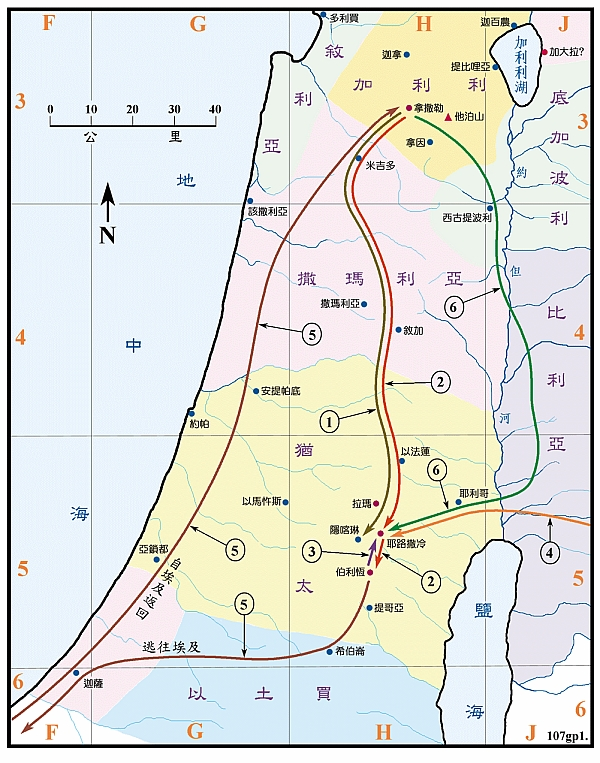
\includegraphics[width=140mm]{ZongJie/SiFuYin/figs/p107} 
\end{figure}



\subsubsection{天使向馬利亞顯現預言耶穌生}
\begin{table}[H]
\centering
\begin{tabular}{p{17.93em}|p{6.07em}|c|c|l|c} \toprule
 事 件   & 地 點   & \multicolumn{1}{p{5em}|}{太} & \multicolumn{1}{p{4.215em}|}{可} & \multicolumn{1}{p{4.215em}|}{路} & \multicolumn{1}{p{4.215em}}{約} \\
\midrule
太初之道是神,生命之真光在他裡&&\multicolumn{1}{p{4.215em}|}{}& & &1:1-4,9\\\midrule 
接待他信他名的人做神的兒女&&\multicolumn{1}{p{4.215em}|}{}& & &1:12-13\\\midrule 
道成肉身父獨生子之光有恩典有真理&&\multicolumn{1}{p{4.215em}|}{}& & &1:14,16-18\\\midrule 
黑暗/自己人不接受光,世界不識他&&\multicolumn{1}{p{4.215em}|}{}& & &1:5,10-11\\\midrule 
亞伯拉罕後裔大衛子孫耶穌父系家譜&&\multicolumn{1}{p{4.215em}|}{1:1-17}& & &  \\\midrule 
路加自序&提阿非羅&       &       & \multicolumn{1}{p{4.215em}|}{1:1-4} &  \\\midrule 
天使向撒迦利亞顯現預言施洗約翰生& 耶路撒冷  &       &       & \multicolumn{1}{p{4.215em}|}{1:5-25} &  \\\midrule 

第六個月天使向馬利亞顯現預言耶穌生& 拿撒勒   & \multicolumn{1}{l|}{1:18} &       & \multicolumn{1}{p{4.215em}|}{1:26-38} &  \\\midrule

馬利亞訪以利沙伯 & 希伯侖隱喀琳   &       &       & \multicolumn{1}{p{4.215em}|}{1:39-56} &  \\\midrule

主的使者夢中向約瑟顯現命其娶馬利亞& 拿撒勒   & \multicolumn{1}{p{5em}|}{1:19-25上} &       &       &  \\\midrule

施洗約翰誕生 & 希伯侖   &       &       & \multicolumn{1}{p{4.215em}|}{1:57-66} &  \\\midrule

撒迦利亞說預言 & 希伯侖   &       &       & \multicolumn{1}{p{4.215em}|}{1:67-79} &  \\\midrule

施洗約翰漸長 & 猶太曠野  &       &       & 1:80 &  \\ \bottomrule
\end{tabular}%
\caption{耶穌誕生前}
  \label{tab:addlabel}%
\end{table}%





\subsubsection{父系家譜}
\begin{forest}
  for tree={
    child anchor=west,
    parent anchor=east,
    grow=east,
    draw,
    anchor=west,
    edge path={
      \noexpand\path[\forestoption{edge}]
        (.child anchor) -| +(-5pt,0) -- +(-5pt,0) |-
        (!u.parent anchor)\forestoption{edge label};
    },
  }
  [亞伯拉罕[以撒[雅各[猶大[法勒斯[希斯崙[亞蘭]]][謝拉]][\textcolor{red}{他瑪氏}]]]]
  ]
\end{forest}

\begin{forest}
  for tree={
    child anchor=west,
    parent anchor=east,
    grow=east,
    draw,
    anchor=west,
    edge path={
      \noexpand\path[\forestoption{edge}]
        (.child anchor) -| +(-5pt,0) -- +(-5pt,0) |-
        (!u.parent anchor)\forestoption{edge label};
    },
  }
[亞米拿達[拿順[撒門[波阿斯[俄備得[耶西[大衛王]]]][\textcolor{red}{路得氏}]][\textcolor{red}{喇合氏}]] 
 ]
\end{forest}
\newline

\begin{forest}
  for tree={
    child anchor=west,
    parent anchor=east,
    grow=east,
    draw,
    anchor=west,
    edge path={
      \noexpand\path[\forestoption{edge}]
        (.child anchor) -| +(-5pt,0) -- +(-5pt,0) |-
        (!u.parent anchor)\forestoption{edge label};
    },
  }
[大衛[所羅門[羅波安[亞比雅[亞撒[約沙法[約蘭][亚她利雅]]]]]][\textcolor{red}{烏利亞的妻子，拔士巴}]
 ]
\end{forest}
\newline

\begin{forest}
  for tree={
    child anchor=west,
    parent anchor=east,
    grow=east,
    draw,
    anchor=west,
    edge path={
      \noexpand\path[\forestoption{edge}]
        (.child anchor) -| +(-5pt,0) -- +(-5pt,0) |-
        (!u.parent anchor)\forestoption{edge label};
    },
  }
[約蘭[烏西亞[約坦[亞哈斯[希西家[瑪拿西[亞們[約西亞]]]]]]]
 ]
\end{forest}
\newline


\begin{forest}
  for tree={
    child anchor=west,
    parent anchor=east,
    grow=east,
    draw,
    anchor=west,
    edge path={
      \noexpand\path[\forestoption{edge}]
        (.child anchor) -| +(-5pt,0) -- +(-5pt,0) |-
        (!u.parent anchor)\forestoption{edge label};
    },
  }
[耶哥尼雅[撒拉鐵[所羅巴伯[亞比玉[以利亞敬[亞所[撒督]]]]]] 
 ]
\end{forest}
%\newline

\begin{forest}
  for tree={
    child anchor=west,
    parent anchor=east,
    grow=east,
    draw,
    anchor=west,
    edge path={
      \noexpand\path[\forestoption{edge}]
        (.child anchor) -| +(-5pt,0) -- +(-5pt,0) |-
        (!u.parent anchor)\forestoption{edge label};
    },
  }
[亞金[以律[以利亞撒[馬但[雅各[約瑟[耶穌][\textcolor{red}{馬利亞}]]]]]] 
 ]
\end{forest}


\subsubsection{母系家譜} 
\begin{forest}
  for tree={
    child anchor=west,
    parent anchor=east,
    grow=east,
    draw,
    anchor=west,
    edge path={
      \noexpand\path[\forestoption{edge}]
        (.child anchor) -| +(-5pt,0) -- +(-5pt,0) |-
        (!u.parent anchor)\forestoption{edge label};
    },
  }
[神的兒子亞當[塞特[以挪士[該南[瑪勒列[雅列[以諾[瑪土撒拉]][與神同行]]]]]]] 
 ]
\end{forest}
\newline

\begin{forest}
  for tree={
    child anchor=west,
    parent anchor=east,
    grow=east,
    draw,
    anchor=west,
    edge path={
      \noexpand\path[\forestoption{edge}]
        (.child anchor) -| +(-5pt,0) -- +(-5pt,0) |-
        (!u.parent anchor)\forestoption{edge label};
    },
  }
[瑪土撒拉[拉麥[挪亞[閃[亞法撒[沙拉[希伯[法勒[拉吳[西鹿[拿鶴]]]]]]]][含][雅弗]]]] 
 ]
\end{forest}
\newline

\begin{forest}
  for tree={
    child anchor=west,
    parent anchor=east,
    grow=east,
    draw,
    anchor=west,
    edge path={
      \noexpand\path[\forestoption{edge}]
        (.child anchor) -| +(-5pt,0) -- +(-5pt,0) |-
        (!u.parent anchor)\forestoption{edge label};
    },
  }
[拿鶴[他拉[亞伯蘭[以撒[雅各[猶大[法勒斯[希斯崙[亞蘭[亞米拿達]]]]]]]][拿鶴[彼土利[\textcolor{red}{利百加(以撒的妻子)}][拉班[\textcolor{red}{拉結}][\textcolor{red}{利亞}]]]][哈蘭[羅得][\textcolor{red}{密迦(拿鶴的妻子)}]][\textcolor{red}{撒萊(亞伯蘭的妻子)}]]] 
 ]
\end{forest}
\newline




\begin{forest}
  for tree={
    child anchor=west,
    parent anchor=east,
    grow=east,
    draw,
    anchor=west,
    edge path={
      \noexpand\path[\forestoption{edge}]
        (.child anchor) -| +(-5pt,0) -- +(-5pt,0) |-
        (!u.parent anchor)\forestoption{edge label};
    },
  }
[亞米拿達[拿順[撒門[波阿斯[俄備得[耶西[大衛[拿單[瑪達他[買南]]]]]]]]]] 
 ]
\end{forest}
\newline

\begin{forest}
  for tree={
    child anchor=west,
    parent anchor=east,
    grow=east,
    draw,
    anchor=west,
    edge path={
      \noexpand\path[\forestoption{edge}]
        (.child anchor) -| +(-5pt,0) -- +(-5pt,0) |-
        (!u.parent anchor)\forestoption{edge label};
    },
  }
[買南[米利亞[以利亞敬[約南[約瑟[猶大[西緬[利未[瑪塔[約令[以利以謝]]]]]]]]]]] 
 ]
\end{forest}
\newline

\begin{forest}
  for tree={
    child anchor=west,
    parent anchor=east,
    grow=east,
    draw,
    anchor=west,
    edge path={
      \noexpand\path[\forestoption{edge}]
        (.child anchor) -| +(-5pt,0) -- +(-5pt,0) |-
        (!u.parent anchor)\forestoption{edge label};
    },
  }
[以利以謝[約細[珥[以摩當[哥桑[亞底[麥基[尼利[撒拉鐵[所羅巴伯]]]]]]]]]]]] 
 ]
\end{forest}
\newline

\begin{forest}
  for tree={
    child anchor=west,
    parent anchor=east,
    grow=east,
    draw,
    anchor=west,
    edge path={
      \noexpand\path[\forestoption{edge}]
        (.child anchor) -| +(-5pt,0) -- +(-5pt,0) |-
        (!u.parent anchor)\forestoption{edge label};
    },
  }
[所羅巴伯[利撒[約亞拿[猶大[約瑟[西美[瑪他提亞[瑪押[拿該[以斯利]]]]]]]]]]]] 
 ]
\end{forest}
\newline

\begin{forest}
  for tree={
    child anchor=west,
    parent anchor=east,
    grow=east,
    draw,
    anchor=west,
    edge path={
      \noexpand\path[\forestoption{edge}]
        (.child anchor) -| +(-5pt,0) -- +(-5pt,0) |-
        (!u.parent anchor)\forestoption{edge label};
    },
  }
[以斯利[拿鴻[亞摩斯[瑪他提亞[約瑟[雅拿[麥基[利未[瑪塔[希里[馬利亞]]]]]]]]]]] 
 ]
\end{forest}

%\subsection{家譜中的女性}
%\subsubsection{他瑪（猶大）}
%\subsubsection{喇合（撒門）}
%\subsubsection{路得（波阿斯）}
%\subsubsection{拔士巴（大衛）}
%\subsubsection{瑪利亞（約瑟）}


%\subsection{夢中的啟示}
\subsubsection{約瑟的四個夢}

\begin{table}[H]
  \centering
    \begin{tabular}{p{6.em}|p{22.2em}|p{11.7em}|p{6.em}}
    \toprule
     \textcolor[rgb]{ .267,  .447,  .769}{\textbf{做夢背景}} 
    & \textcolor[rgb]{ .267,  .447,  .769}{\textbf{夢的內容}}
       & \textcolor[rgb]{ .267,  .447,  .769}{\textbf{人的反應}} 
    %& \textcolor[rgb]{ .267,  .447,  .769}{\textbf{經文}}
     & \textcolor[rgb]{ .267,  .447,  .769}{\textbf{應驗經文}} \\    
  \midrule    
    馬利亞就從聖靈懷了孕  &有主的使者向他\textbf{夢中顯現}，說：「 大衛的子孫約瑟，不要怕！只管娶過你的妻子馬利亞來，因他所懷的孕是從聖靈來的。他將要生一個兒子，你要給他起名叫耶穌，因他要將自己的百姓從罪惡裡救出來。」  &約瑟醒了,起來,就遵著主使者的吩咐把妻子娶過來;只是沒有和他同房,等他生了兒子,就給他起名叫耶穌 &「必有童女懷孕生子；人要稱他的名為以馬內利。」 \\ %&1:20
  \midrule  
     博士去後& 有主的使者向約瑟\textbf{夢中顯現}，說：「起來！帶著小孩子同他母親逃往埃及，住在那裡，等我吩咐你；因為希律必尋找小孩子，要除滅他。」 & 約瑟就起來，夜間帶著小孩子和他母親往埃及去住在那裡，直到希律死了。 &「我從埃及召出我的兒子來。」\\%&2:13-15
    \midrule  
希律死了以後    &有主的使者在埃及向約瑟\textbf{夢中顯現}，說：「起來！帶著小孩子和他母親往以色列地去，因為要害小孩子性命的人已經死了。」 &約瑟就起來，把小孩子和他母親帶到以色列地去&\\%&2:20-23
    \midrule  
   亞基老作猶太王，約瑟怕&又在\textbf{夢中被主指示}，便往加利利境內去了 &到了一座城，名叫拿撒勒，就住在那裡。 &他將稱為拿撒勒人\\%&2:22, 23
    \midrule 
    \bottomrule
    \end{tabular}%
  \label{tab:addlabel}%
   \caption{約瑟的四個夢}
\end{table}%

\subsubsection{博士夢中的啟示}
\begin{table}[H]
  \centering
    \begin{tabular}{p{4em}|p{7.2em}|p{6.7em}|p{22.em}}
    \toprule
     \textcolor[rgb]{ .267,  .447,  .769}{\textbf{做夢背景}} 
    & \textcolor[rgb]{ .267,  .447,  .769}{\textbf{夢的內容}}
       & \textcolor[rgb]{ .267,  .447,  .769}{\textbf{人的反應}} 
     & \textcolor[rgb]{ .267,  .447,  .769}{\textbf{應驗經文}} \\ \midrule        
  博士拜完小孩子  &  \textbf{夢中被主指示}不要回去見希律 & 就從別的路回本地去了。&在拉瑪聽見號咷大哭的聲音，是拉結哭他兒女，不肯受安慰，因為他們都不在了\\ %&2:11, 12
    \bottomrule
    \end{tabular}%
  \label{tab:addlabel}%
   \caption{博士夢中的啟示}
\end{table}%

%\newpage
\subsubsection{耶穌降生}

%\begin{figure}%
%    \centering
%    \includegraphics[height=10cm]{SiFuYin/fig/jesusbegin}
 %   \label{fig:example}%
%\end{figure}


\begin{table}[H]
  \centering
    \begin{tabular}{p{8.93em}c|p{5.07em}|r|c|p{5.215em}|c}
    \toprule
    \multicolumn{2}{p{14.575em}|}{事 件}  & 地 點   & \multicolumn{1}{p{4.215em}|}{馬太福音} & \multicolumn{1}{p{4.215em}|}{馬可福音} & 路加福音  & \multicolumn{1}{p{4.215em}}{約翰福音} \\
    \midrule
    \multicolumn{2}{p{14.575em}|}{耶穌基督降生} & 伯利恒   & \multicolumn{1}{p{4.215em}|}{2:1上} &       & 2:1-7 &  \\
    \midrule
%    \multicolumn{2}{p{14.575em}|}{天使傳報喜訊} & 伯利恒   &       &       & 2:8-14 &  \\
%    \midrule
    \multicolumn{2}{p{14.575em}|}{\textcolor{red}{當天晚上}天使報訊，牧羊人拜訪} & 伯利恒   &       &       & 2:8-20 &  \\
    \midrule
    \multicolumn{2}{p{14.575em}|}{\textcolor{red}{第八天}受割禮受割禮與起名} & 伯利恒   & \multicolumn{1}{p{4.215em}|}{1:25下} &       & \multicolumn{1}{l|}{2:21} &  \\
    \midrule
    \multicolumn{1}{l|}{\multirow{2}[4]{*}{耶穌家譜}} & \multicolumn{1}{p{6.645em}|}{父系家譜} & \multicolumn{1}{r|}{} & \multicolumn{1}{p{4.215em}|}{1:1-17} &       & \multicolumn{1}{r|}{} &  \\
    
\cmidrule{2-7}    \multicolumn{1}{c|}{} & \multicolumn{1}{p{6.645em}|}{母系家譜} & \multicolumn{1}{r|}{} &       &       & 3:23下-38 &  \\  \midrule

%\multicolumn{1}{c|}{\multirow{3}[6]{*}{第四十天去聖}} & \multicolumn{1}{p{6.645em}|}{a.行潔淨的禮} & 耶路撒冷  &       &       & 2:22-24 &  \\
\multicolumn{1}{c|}{\textcolor{red}{第四十天}去聖} & \multicolumn{1}{p{6.645em}|}{a.行潔淨的禮} & 耶路撒冷  &       &       & 2:22-24 &  \\
\cmidrule{2-7}    \multicolumn{1}{c|}{殿做奉獻禮,} & \multicolumn{1}{p{6.645em}|}{b.西面的稱頌} & 耶路撒冷  &       &       & 2:25-35 &  \\
\cmidrule{2-7}    \multicolumn{1}{c|}{耶穌被獻給神} & \multicolumn{1}{p{6.645em}|}{c.亞拿的講解} & 耶路撒冷  &       &       & 2:36-38 &  \\ \midrule

 \multicolumn{2}{p{14.575em}|}{耶穌\textcolor{red}{两岁前}受幾個東方博士朝拜} & 伯利恒   & \multicolumn{1}{p{4.215em}|}{2:1下-12} &       & \multicolumn{1}{r|}{} &  \\ \midrule

\multicolumn{2}{p{14.575em}|}{約瑟帶耶穌等逃往埃及} & 埃及    & \multicolumn{1}{p{4.215em}|}{2:13-15} &       & \multicolumn{1}{r|}{} &  \\
    \midrule
    \multicolumn{2}{p{14.575em}|}{希律屠殺男孩} & 伯利恒   & \multicolumn{1}{p{4.215em}|}{2:16-18} &       & \multicolumn{1}{r|}{} &  \\
    \midrule
    \multicolumn{2}{p{14.575em}|}{約瑟耶穌等返拿撒勒并长大} & 拿撒勒   & \multicolumn{1}{p{4.215em}|}{2:19-23} &       & 2:39下-40 &  \\
    \midrule
    \multicolumn{2}{p{14.575em}|}{耶穌\textcolor{red}{12歲}赴聖殿過節} & 耶路撒冷  &       &       & 2:41-52&  \\
    \bottomrule
    \end{tabular}%
         \caption{耶穌降生及幼年}
  \label{tab:addlabel}%
\end{table}%


\subsubsection{耶穌受洗}
\begin{table}[H]
  \centering 
    \begin{tabular}{p{7.645em}c|p{4.855em}|p{4.215em}|p{4.215em}|p{4.215em}|l}
    \toprule
    \multicolumn{2}{p{20.075em}|}{事 件} & 地 點   & 馬太福音  & 馬可福音  & 路加福音  & \multicolumn{1}{p{4.215em}}{約翰福音} \\ \midrule

\multicolumn{2}{p{20.075em}|}{神的話臨到施洗約翰} & 猶太曠野  & \multicolumn{1}{r|}{} & \multicolumn{1}{r|}{} & 3:1-2 &  \\ \midrule

\multicolumn{1}{c|}{\multirow{5}[10]{*}{施洗約翰的工作}} & \multicolumn{1}{p{13.43em}|}{a.他的工作:爲光作見證} & \multicolumn{1}{l|}{} & \multicolumn{1}{r|}{} & \multicolumn{1}{l|}{} & \multicolumn{1}{r|}{} & \multicolumn{1}{p{4.215em}}{1:6-8} \\
\cmidrule{2-7}    \multicolumn{1}{c|}{} & \multicolumn{1}{p{13.43em}|}{b.他的資訊:天國進了} & \multicolumn{1}{r|}{} & 3:1-2 & \multicolumn{1}{r|}{} & \multicolumn{1}{r|}{} &  \\
\cmidrule{2-7}    \multicolumn{1}{c|}{} & \multicolumn{1}{p{13.43em}|}{c.他的職事:傳悔改的洗禮} & \multicolumn{1}{r|}{} & 3:5-6 & 1:4-5 & \multicolumn{1}{l|}{3:3,18} &  \\
\cmidrule{2-7}    \multicolumn{1}{c|}{} & \multicolumn{1}{p{13.43em}|}{d.他的衣食} & \multicolumn{1}{r|}{} & \multicolumn{1}{l|}{3:4} & \multicolumn{1}{l|}{1:6} & \multicolumn{1}{r|}{} &  \\
\cmidrule{2-7}    \multicolumn{1}{c|}{} & \multicolumn{1}{p{13.43em}|}{e.這是應驗先知預言} & \multicolumn{1}{r|}{} & \multicolumn{1}{l|}{3:3} & 1:1-3 & 3:4-6 &  \\\midrule

    \multicolumn{2}{p{20.075em}|}{約翰警告法利賽人和撒都該人悔改} & 約但河   & 3:7-10 & \multicolumn{1}{r|}{} & 3:7-9&  \\ \midrule

 \multicolumn{2}{p{20.075em}|}{約翰劝眾人分衣裳食物给穷人} & 約但河   &  & \multicolumn{1}{r|}{} & 3:10-11 &  \\ \midrule
\multicolumn{2}{p{20.075em}|}{約翰劝稅吏不要多取} & 約但河   &  & \multicolumn{1}{r|}{} & 3:12-13&  \\ \midrule
\multicolumn{2}{p{20.075em}|}{約翰劝兵丁不要以強暴待人} & 約但河   &  & \multicolumn{1}{r|}{} & 3:14&  \\ \midrule
\multicolumn{2}{p{20.075em}|}{約翰向法利賽差的人说其是曠野人聲} & 伯大巴喇   & & &  & 1:19-24 \\  \midrule

\multicolumn{2}{p{20.075em}|}{約翰用水施洗,在我以後來的用聖靈與火施洗} & 約但河   & 3:11-12 & 1:7-8 & 3:15-17 & 1:25-28\\  \midrule
%\multicolumn{2}{p{20.075em}|}{約翰勸百姓悔改向他們傳福音} & 約但河   &&& 3:18 & \\  \midrule
\multicolumn{2}{p{20.75em}|}{次日約翰見主说,神羔羊在我以後來本在我以前} & 約但河   &&& &3:15,29-31\\  \midrule
\multicolumn{2}{p{20.075em}|}{耶穌受浸時禱告} & 約但河   & & & 3:21& \\\midrule
\multicolumn{2}{p{20.075em}|}{耶穌受浸時聖靈降臨} & 約但河   & 3:13-16& 1:9-10 & 3:22a &1:32-34 \\\midrule
\multicolumn{2}{p{20.075em}|}{耶穌受浸時天上聲音說"這是我愛子所喜悅的"} & 約但河   & 3:17 & 1:11 & 3:22b & \\\midrule


    \multicolumn{2}{p{20.075em}|}{被聖靈引到曠野受魔鬼試探四十天} & 猶太曠野  & 4:1-10 & 1:12-13a & 4:1-13 &  \\\midrule
\multicolumn{2}{p{20.075em}|}{魔鬼離了耶穌，有天使來伺候他} & 猶太曠野  & 4:11 & 1:13b &&  \\
    \bottomrule
    \end{tabular}%
     \caption{預備期}
  \label{tab:addlabel}%
\end{table}%


\subsubsection{耶穌受試探}
\begin{table}[H]
  \centering
    \begin{tabular}{p{11em}|p{18.em}|p{16.5em}}
    \toprule
     \textcolor[rgb]{ .267,  .447,  .769}{\textbf{試探地點}} 
    & \textcolor[rgb]{ .267,  .447,  .769}{\textbf{魔鬼試探內容}}    
     & \textcolor[rgb]{ .267,  .447,  .769}{\textbf{耶穌回答經文}} \\    
  \midrule    
    曠野禁食四十晝夜，後來就餓了  
    &你若是神的兒子，可以吩咐這些石頭變成食物。 
    &經上記著說：人活著，不是單靠食物，乃是靠神口裡所出的一切話。(申8:3) \\ %&1:20
    \midrule  
  魔鬼就帶他進了聖城，叫他站在殿頂（頂原文作翅）上 
  &  你若是神的兒子，可以跳下去，因為經上記著：主要為你吩咐他的使者用手托著你，免得你的腳碰在石頭上。(詩91:11-12)
  &經上又記著說：『不可試探主你的神。』(申6:16) \\   %&2:11, 12
  \midrule
  魔鬼又帶他上了一座最高的山，將世上的萬國與萬國的榮華都指給他看
  & 你若俯伏拜我，我就把這一切都賜給你。
  & 撒但（撒但是抵擋的意思,魔鬼別名），退去吧！因為經上記著說：當拜主你的神，單要事奉他(申6:13)。 \\% &2:13-15    
    \bottomrule
    \end{tabular}%
  \label{tab:addlabel}%
   \caption{耶穌受試探}
\end{table}%


\subsection{耶穌的服事}

\subsubsection{施洗约翰被囚前\href{http://biblegeography.holylight.org.tw/index/condensedbible_map_detail?m_id=108}{(耶稣受洗初期服事路线)}}
\begin{table}[H]
\centering
\begin{tabular}{p{6.45em}|c|p{4.785em}|r|p{3.em}|p{3.23em}|p{3.5em}}\toprule

\multicolumn{2}{p{20.5em}|}{事 件} & 地 點& \multicolumn{1}{p{3.23em}|}{太} & \multicolumn{1}{p{3.23em}|}{可}    & \multicolumn{1}{p{3.23em}|}{路} & \multicolumn{1}{p{3.5em}}{約} \\\midrule\midrule

\multicolumn{2}{p{20.5em}|}{耶穌約三十歲開頭傳道} & \multicolumn{1}{p{5.355em}|}{加利利} &\multicolumn{1}{p{4.145em}|}{}&\multicolumn{1}{p{3.85em}|}{}&\multicolumn{1}{p{3.5em}|}{3:23}& \\ \midrule

\multirow{5}[8]{*}{五門徒跟從耶穌} & \multicolumn{1}{p{13.355em}|}{次日約翰門徒(約翰/安德烈)} & \multirow{4}[8]{*}{約但河} & & && 1:35-39 \\

\cmidrule{2-2}\cmidrule{4-7}    \multicolumn{1}{c|}{} & \multicolumn{1}{p{13.355em}|}{安德烈领西門歸主,改名彼得} & \multicolumn{1}{c|}{} & & & & 1:40-42 \\

\cmidrule{2-2}\cmidrule{4-7}    \multicolumn{1}{c|}{} & \multicolumn{1}{p{13.355em}|}{又次日去加利利路上呼召腓力} & \multicolumn{1}{c|}{} &  & & & 1:43-44 \\

\cmidrule{2-2}\cmidrule{4-7}\multicolumn{1}{c|}{} & \multicolumn{1}{p{13.355em}|}{伯賽大人腓力领拿但業歸主}&\multicolumn{1}{c|}{}&&&&1:45-48\\

\cmidrule{2-2}\cmidrule{4-7}\multicolumn{1}{c|}{} & \multicolumn{1}{p{13.355em}|}{迦拿人拿但業认耶稣为神兒子}&\multicolumn{1}{c|}{}&&&&1:49-51\\\midrule

\multicolumn{2}{p{20.5em}|}{第一個神迹:婚宴變水為酒}&迦拿&&&& 2:1-11\\\midrule

\multicolumn{2}{p{20.5em}|}{耶穌第一次與門徒去迦百農住了不多幾日}&迦百農&&&&2:12\\\midrule

耶穌潔淨聖殿 & 
\multicolumn{1}{c|}{\multirow{3}[6]{*}{第一个逾越節}} &
\multicolumn{1}{l|}{\multirow{3}[6]{*}{耶路撒冷}}&&&&2:13-17\\

\cmidrule{1-1}\cmidrule{4-7}三日再建圣殿&&&&&& 2:18-22 \\
\cmidrule{1-1}\cmidrule{4-7} 行好些神迹 &（共四个逾越节）&&&&& 2:23-25 \\
\cmidrule{1-1}\cmidrule{4-7} 尼哥底母夜访&&&&&&3:1-21\\\midrule

\multicolumn{2}{p{20.5em}|}{耶穌的門徒給人施浸} & \multicolumn{1}{p{5.355em}|}{猶太地} &       &       &       & 3:22\\\midrule

\multicolumn{2}{p{20.5em}|}{施洗\textcolor{red}{約翰}最後的見證:他必興旺我必衰微} & \multicolumn{1}{p{5.355em}|}{撒冷的哀嫩} &       &       &       & 3:23-36 \\ \midrule

\multicolumn{2}{p{20.5em}|}{法利賽人見主施洗比約翰多,耶穌離開猶太地} & \multicolumn{1}{p{5.355em}|}{猶太地} &       &       &       & 4:1-3a\\\midrule

\multicolumn{2}{p{20.5em}|}{耶穌與撒馬利亞婦人谈用心靈和誠實拜父傳道} & 
\multicolumn{1}{l|}{\multirow{2}[6]{*}{敘加}} &       &       &       & 4:3b-30\\

\cmidrule{1-2}\cmidrule{4-7}\multicolumn{2}{p{20.5em}|}{對門徒讲:食物是遵行父的旨意，莊稼熟了} &  &       &       &       & 4:31-38\\ 

\cmidrule{1-2}\cmidrule{4-7}\multicolumn{2}{p{20.5em}|}{福音在敘加傳開} &  &       &       &       & 4:39-42 \\ \midrule

\multicolumn{2}{p{20.5em}|}{加利利人見主在耶京所行的就接待他} & \multicolumn{1}{p{5.355em}|}{迦拿} &       &       &       & 4:43-45 \\ \midrule
\multicolumn{2}{p{20.5em}|}{第二個神迹:在迦拿醫治大臣兒子(在迦百農)} & \multicolumn{1}{p{5.355em}|}{迦拿} &       &       &       & 4:46-54 \\ \midrule
\end{tabular}
\caption{两个神迹/3(耶稣)+1(约翰)讲道}
\end{table}

\begin{figure}[H]
\centering
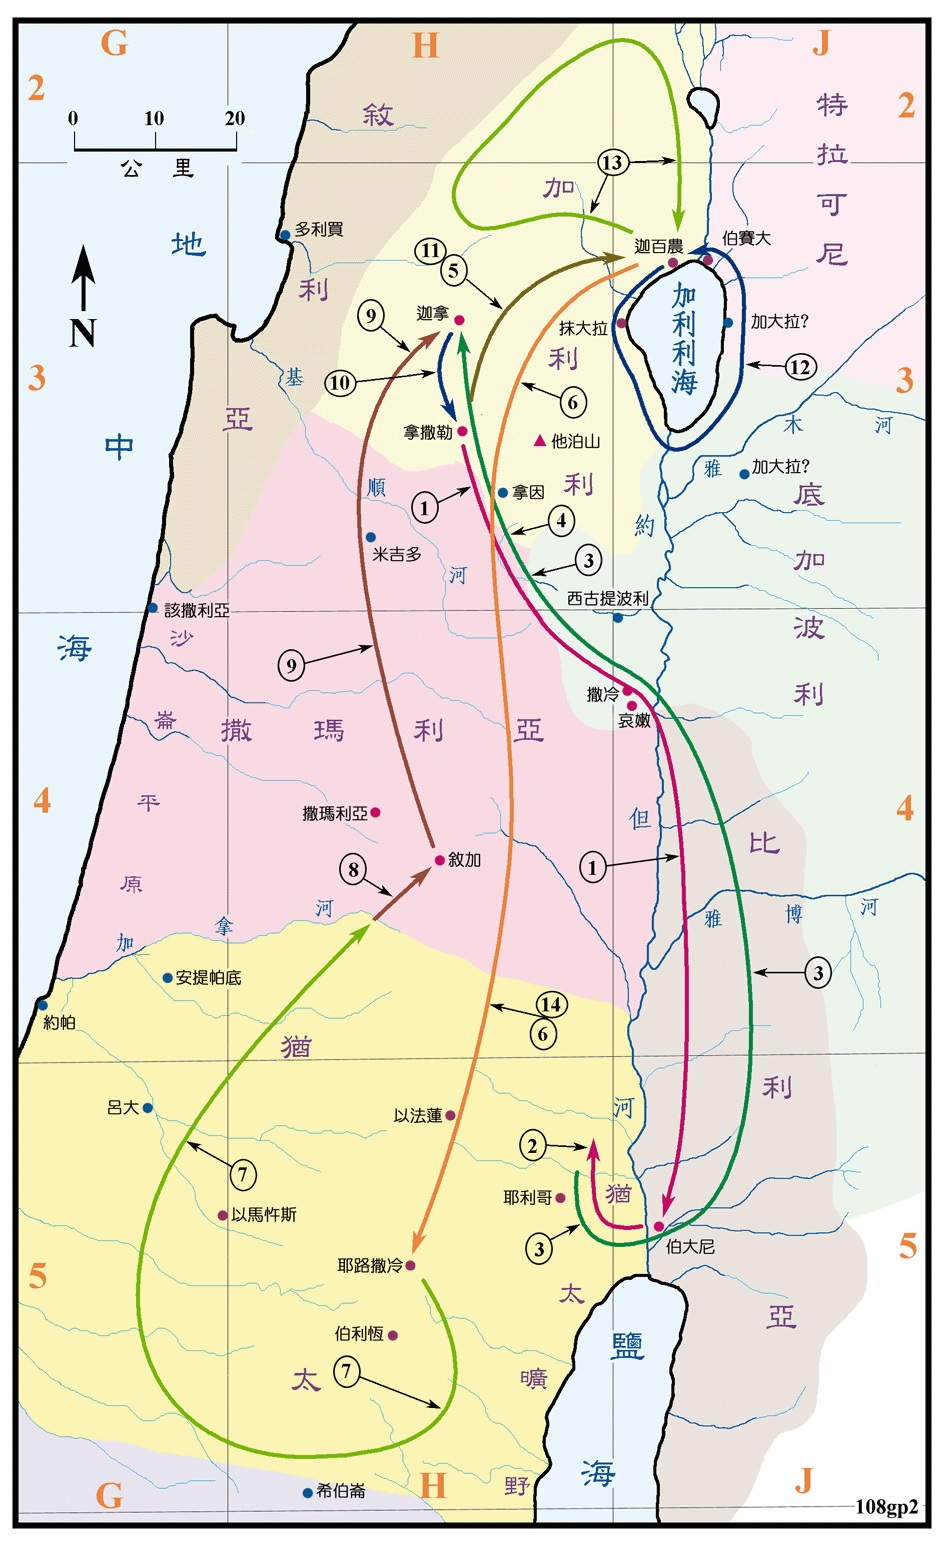
\includegraphics[width=150mm]{ZongJie/SiFuYin/figs/jesustripYouth} 
\caption{初期服事路线}
\end{figure}

\subsubsection{施洗约翰被囚后开始呼召门徒\href{http://biblegeography.holylight.org.tw/index/condensedbible_map_detail?m_id=109}{(揀選门徒后的服事)}}

\begin{table}[H]\centering 
\begin{tabular}{p{6.45em}|c|p{4.785em}|r|p{6.em}|p{3.23em}|p{1.em}}\toprule

\multicolumn{2}{p{20.em}|}{事 件} & 地 點& \multicolumn{1}{p{3.23em}|}{太} & \multicolumn{1}{p{3.23em}|}{可}    & \multicolumn{1}{p{3.23em}|}{路} & \multicolumn{1}{p{1.em}}{約} \\\midrule\midrule

\multicolumn{2}{p{20.em}|}{\textcolor{red}{施洗約翰被囚}} &\multicolumn{1}{p{4.145em}|}{希律王宫} &{4:12/14:3-5} &\multicolumn{1}{p{6em}|}{1:14/6:17-20}&\multicolumn{1}{p{3.5em}|}{3:19-20}& \\ \midrule

%\multicolumn{2}{p{20.5em}|}{耶穌聽見約翰下了監,回加利利在各會堂傳道} & \multicolumn{1}{p{5.355em}|}{加利利} &\multicolumn{1}{p{4.145em}|}{4:12}&&& \\ \midrule


\multicolumn{2}{p{20.em}|}{聽約翰下監安息日照常進會堂念經} & \multicolumn{1}{p{4.355em}|}{拿撒勒} &\multicolumn{1}{p{4.145em}|}{4:12-13a}&&\multicolumn{1}{p{3.5em}|}{4:16-22}&\\\hline

\multicolumn{2}{p{20.em}|}{讲撒勒法寡婦和乃縵被攆出城帶到山崖} & \multicolumn{1}{p{5.355em}|}{拿撒勒山崖} &\multicolumn{1}{p{4.145em}|}{}&&\multicolumn{1}{p{3.5em}|}{4:23-30}&\\\hline



\multicolumn{2}{p{20.em}|}{耶穌开始傳「天國近了你們應當悔改」} & \multicolumn{1}{p{4.355em}|}{迦百農} &\multicolumn{1}{p{4.145em}|}{4:13b-17}&\multicolumn{1}{p{3.85em}|}{1:14-15}&\multicolumn{1}{p{3.5em}|}{4:14-15}&\\\hline
\multicolumn{2}{p{20.em}|}{海邊首次召彼得/安德烈/约翰/雅各} & & \multicolumn{1}{p{4.145em}|}{4:18-22} & \multicolumn{1}{p{4.43em}|}{1:16-20} & &  \\


\cmidrule{1-2}\cmidrule{4-7}\multicolumn{2}{p{20.em}|}{安息日在迦百農會堂裡趕逐汙鬼傳道} &\multicolumn{1}{l|}{\multirow{4}{*}{迦百農}}  &  & \multicolumn{1}{p{4.43em}|}{1:21-28} & \multicolumn{1}{p{3.5em}|}{4:31-37} & \multicolumn{1}{r}{} \\ 

\cmidrule{1-2}\cmidrule{4-7}\multicolumn{2}{p{20.em}|}{安息日在西門家醫彼得岳母熱病} && \multicolumn{1}{p{4.145em}|}{8:14-15} & \multicolumn{1}{p{4.43em}|}{1:29-31} & \multicolumn{1}{p{3.5em}|}{4:38-39} & \multicolumn{1}{r}{} \\ 

\cmidrule{1-2}\cmidrule{4-7}\multicolumn{2}{p{20.em}|}{晚上醫治各樣病人,應驗以賽亞预言} && \multicolumn{1}{p{4.145em}|}{8:16-17} & \multicolumn{1}{p{4.43em}|}{1:32-34} & \multicolumn{1}{p{3.5em}|}{4:40-41} &  \\ 


\cmidrule{1-2}\cmidrule{4-7}\multicolumn{2}{p{20.em}|}{次日晨耶穌到曠野禱告西門等追之} && \multicolumn{1}{p{4.145em}|}{} & \multicolumn{1}{p{4.43em}|}{1:35-38} & \multicolumn{1}{p{3.5em}|}{4:42-43} &  \\ \midrule

\multicolumn{2}{p{20.5em}|}{與門徒周遊傳道醫病,名傳敘利亞} &\multicolumn{1}{l|}{\multirow{2}{*}{加利利}} & \multicolumn{1}{p{4.145em}|}{4:23-24} & \multicolumn{1}{p{4.43em}|}{1:39} & \multicolumn{1}{p{3.5em}|}{4:44} & \\ 

\cmidrule{1-2}\cmidrule{4-7}\multicolumn{2}{p{20.em}|}{人從加利利低加波利耶京猶太約旦河外來} &\multicolumn{1}{l|}{\multirow{2}{*}{}} & \multicolumn{1}{p{4.145em}|}{4:25} & \multicolumn{1}{p{4.43em}|}{} & \multicolumn{1}{p{3.5em}|}{} & \\ 

\cmidrule{1-2}\cmidrule{4-7}\multicolumn{2}{p{20.em}|}{湖边二次召彼得/雅各/約翰得人如得鱼} &  & \multicolumn{1}{p{4.145em}|}{} & \multicolumn{1}{p{4.43em}|}{} & \multicolumn{1}{p{3.5em}|}{5:1-11} &\\

\cmidrule{1-2}\cmidrule{4-7}\multicolumn{2}{p{20.5em}|}{山下的城裡伸手摸,醫治長大痲瘋的人} &  & \multicolumn{1}{p{4.145em}|}{8:1-4} & \multicolumn{1}{p{4.43em}|}{1:40-45} & \multicolumn{1}{p{3.5em}|}{5:12-16} & \multicolumn{1}{c}{} \\ \midrule

\multicolumn{2}{p{20.em}|}{在法利賽人和教法師面前醫四人擡癱子} & \multicolumn{1}{l|}{\multirow{5}{*}{迦百農}}& \multicolumn{1}{p{4.145em}|}{9:1-8} & \multicolumn{1}{p{4.43em}|}{2:1-12} & \multicolumn{1}{p{3.5em}|}{5:17-26} & \\
\cmidrule{1-2}\cmidrule{4-7}  \multicolumn{2}{p{20.em}|}{耶穌召坐在稅關上稅吏利未(馬太)} & & \multicolumn{1}{p{4.145em}|}{9:9} & \multicolumn{1}{p{4.43em}|}{2:13-14} & \multicolumn{1}{p{3.5em}|}{5:27-28} &\\
\cmidrule{1-2}\cmidrule{4-7}\multicolumn{2}{p{20.em}|}{在馬太家坐席法利賽人文士向門徒發怨言} && \multicolumn{1}{p{4.145em}|}{9:10-13} & \multicolumn{1}{p{4.43em}|}{2:15-17} & \multicolumn{1}{p{3.85em}|}{5:29-32} &  \\
\cmidrule{1-2}\cmidrule{4-7}\multicolumn{2}{p{20.em}|}{對約翰門徒和法利賽人論禁食} && \multicolumn{1}{p{4.145em}|}{9:14-15} & \multicolumn{1}{p{4.43em}|}{2:18-20} & \multicolumn{1}{p{3.85em}|}{5:33-35} &\\ 
\cmidrule{1-2}\cmidrule{4-7}\multicolumn{2}{p{20.em}|}{新布補舊衣服,新酒裝在舊皮袋的比喻} && \multicolumn{1}{p{4.145em}|}{9:16-17} & \multicolumn{1}{p{4.43em}|}{2:21-22} & \multicolumn{1}{p{3.5em}|}{5:36-39} &\\ \midrule


\multicolumn{2}{p{20.em}|}{畢士大池醫38年瘫子} & \multicolumn{1}{l|}{\multirow{5}{*}{耶京(更晚?)}}& &  & &\multicolumn{1}{p{3.95em}}{5:1-15}\\
\cmidrule{1-2}\cmidrule{4-7}\multicolumn{2}{p{20.em}|}{猶太人逼迫主犯安息日想杀他}&       &       &       &       & \multicolumn{1}{p{3.95em}}{5:16-18}\\
\cmidrule{1-2}\cmidrule{4-7}\multicolumn{2}{p{20.em}|}{子遵父命，父給子審判權} &       &       &       &       & \multicolumn{1}{p{3.95em}}{5:19-30} \\
\cmidrule{1-2}\cmidrule{4-7}\multicolumn{2}{p{20.em}|}{耶稣的五个見證:約翰/所行/父/聖經/摩西}&       &       &       &       & \multicolumn{1}{p{3.95em}}{5:31-47}\\ \midrule


%\cmidrule{1-2}\cmidrule{4-7}\multicolumn{2}{p{20.5em}|}{對約翰門徒和法利賽人論禁食} && \multicolumn{1}{p{4.145em}|}{9:14-15} & \multicolumn{1}{p{4.43em}|}{2:18-20} & \multicolumn{1}{p{3.85em}|}{5:33-35} &\\ 

\multicolumn{2}{p{12.em}|}{門徒安息日掐麥穗引辯論}&\multicolumn{1}{p{5.3em}|}{從麥地經過} &\multicolumn{1}{p{4.43em}|}{12:1-8}&\multicolumn{1}{p{4.43em}|}{2:23-28}&\multicolumn{1}{p{4.em}|}{6:1-5}& \\  \midrule

\multicolumn{2}{p{12.em}|}{安息日在會堂醫枯右手者}&\multicolumn{1}{p{7.1em}|}{離開麥地進會堂}&\multicolumn{1}{p{4.em}|}{12:9-13}&\multicolumn{1}{p{4.43em}|}{3:1-5}&\multicolumn{1}{p{4.em}|}{6:6-10}& \\ \midrule

\multicolumn{2}{p{15em}|}{法利賽人希律黨人要除滅耶穌}&\multicolumn{1}{p{5.5em}|}{離開會堂}&\multicolumn{1}{p{4.em}|}{12:14}&\multicolumn{1}{p{4.43em}|}{3:6}&\multicolumn{1}{p{4.em}|}{6:11}& \\ \midrule

\multicolumn{2}{p{12.5em}|}{應驗以賽亞的話主僕不爭競}&\multicolumn{1}{p{5.355em}|}{}&\multicolumn{1}{p{4.em}|}{12:15-21}&\multicolumn{1}{p{4.43em}|}{}&\multicolumn{1}{p{4.em}|}{}& \\ \midrule
\end{tabular}

\end{table}


\begin{figure}[H]
\centering
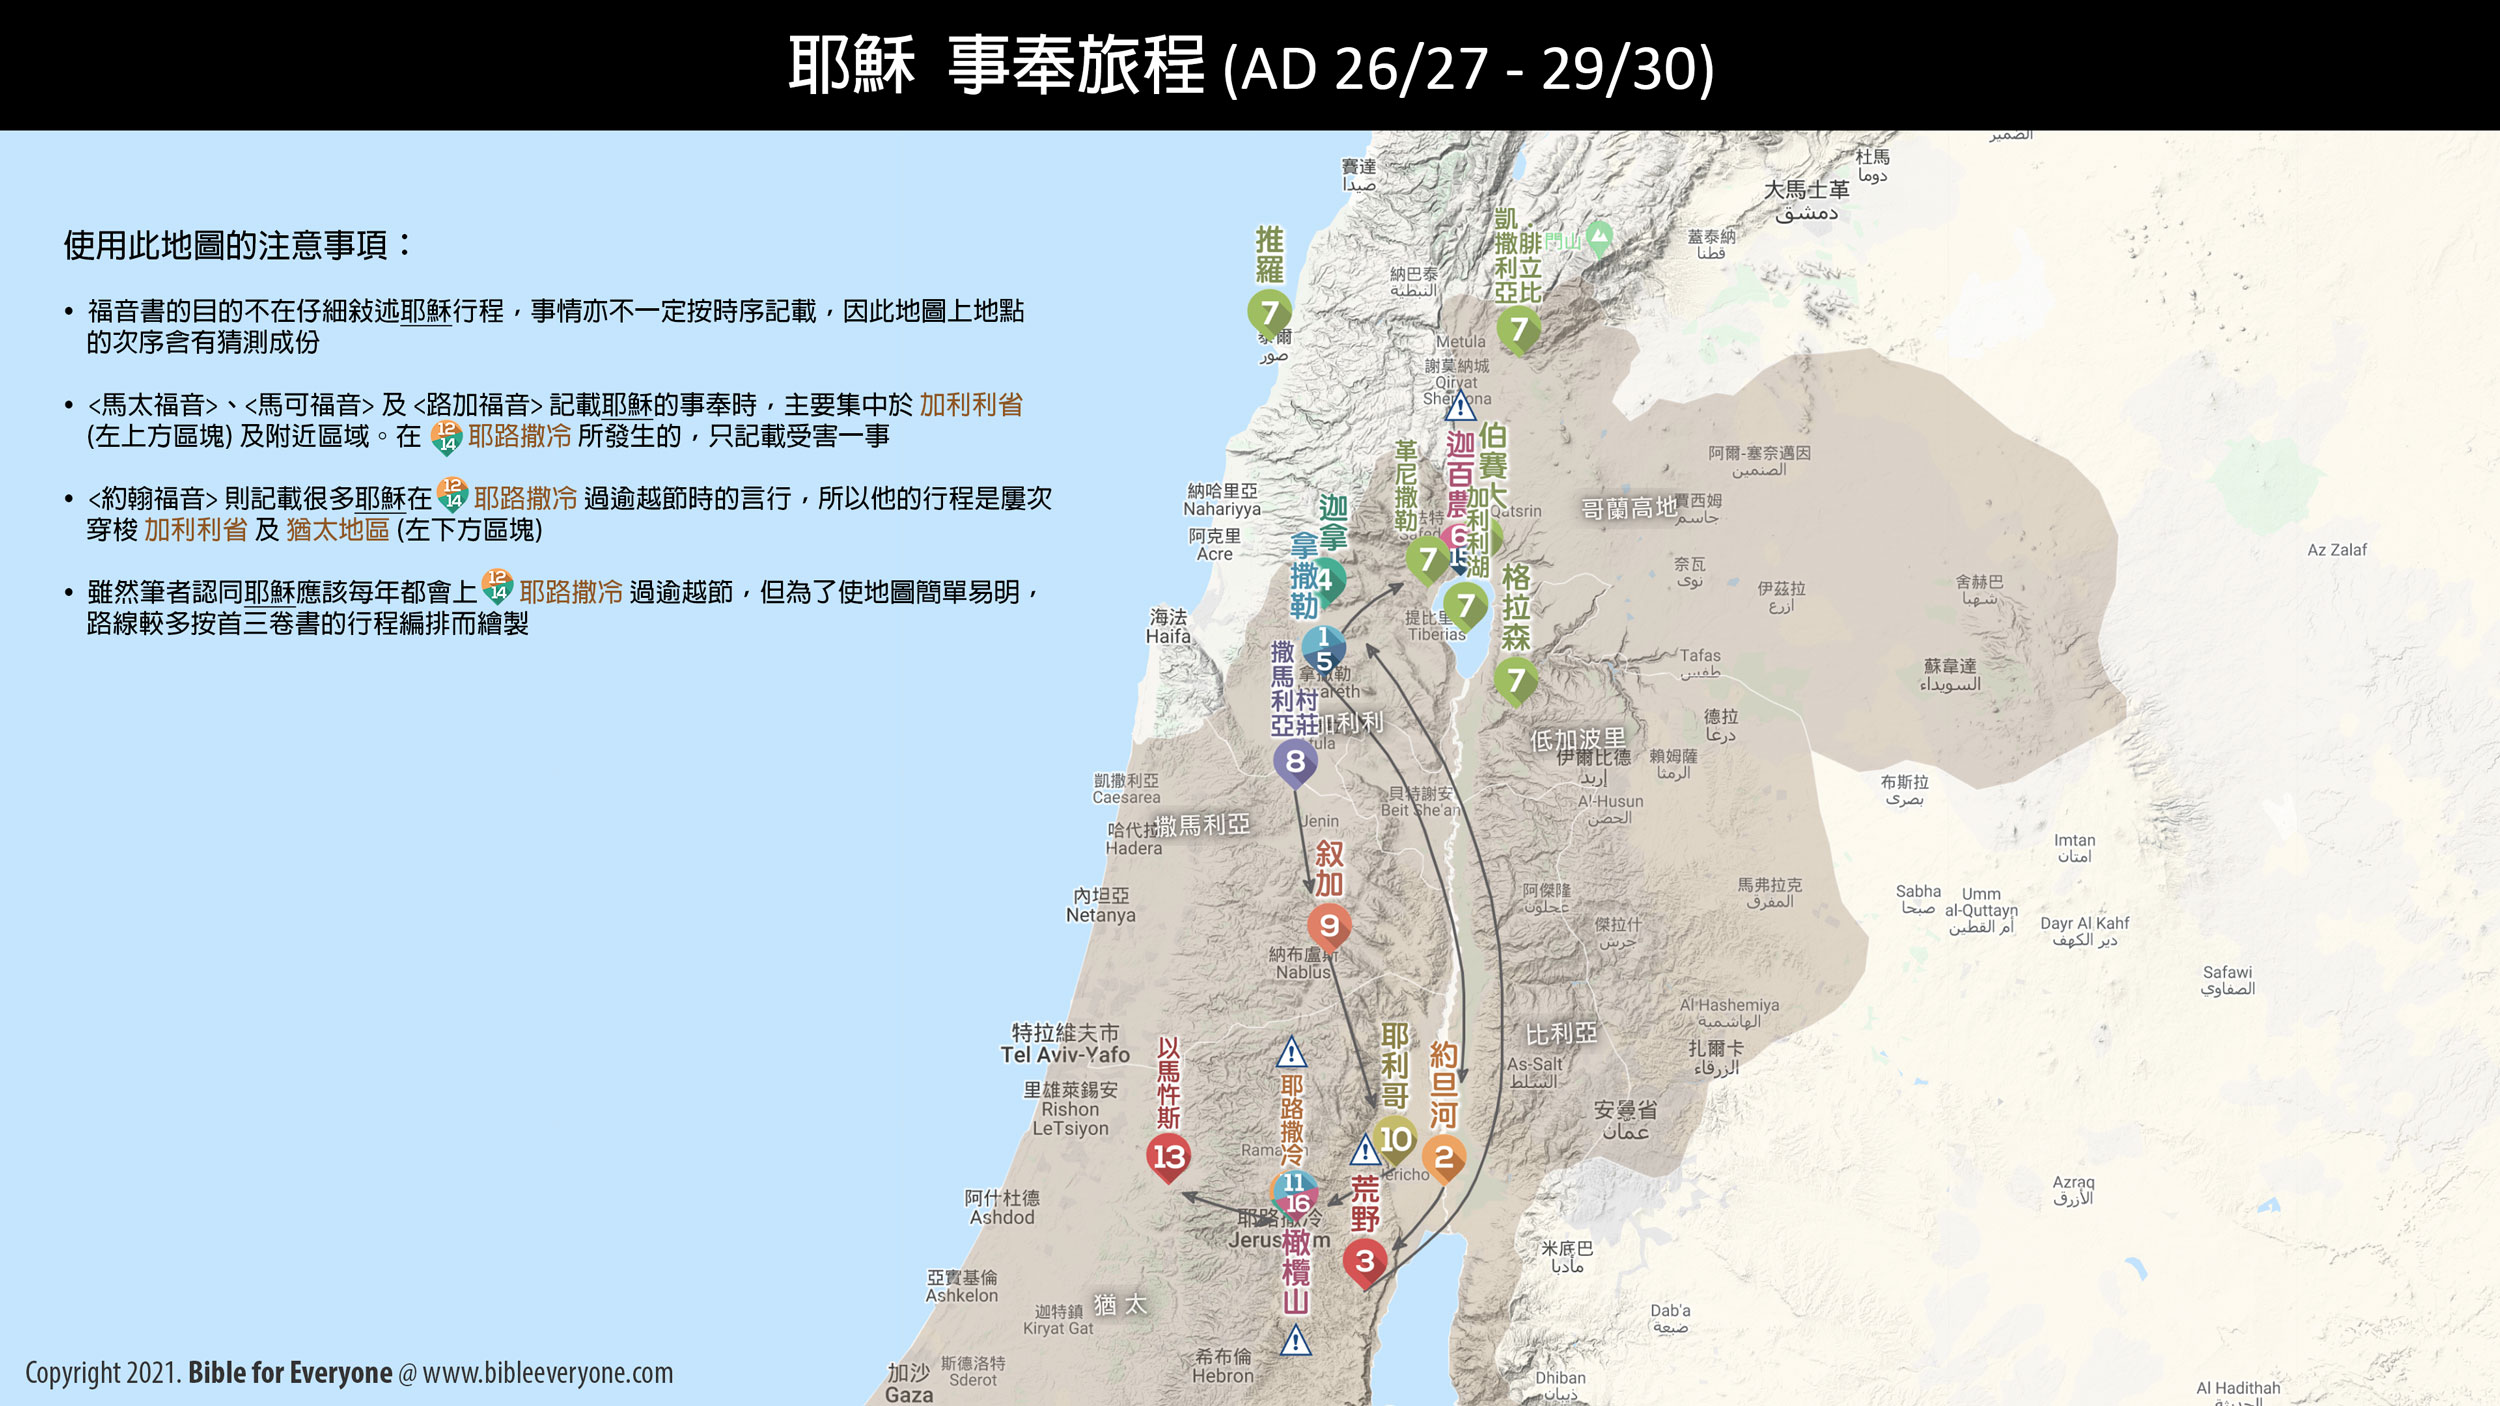
\includegraphics[width=155mm]{ZongJie/SiFuYin/figs/jesustrip} 
\end{figure}

\begin{figure}[H]
\centering
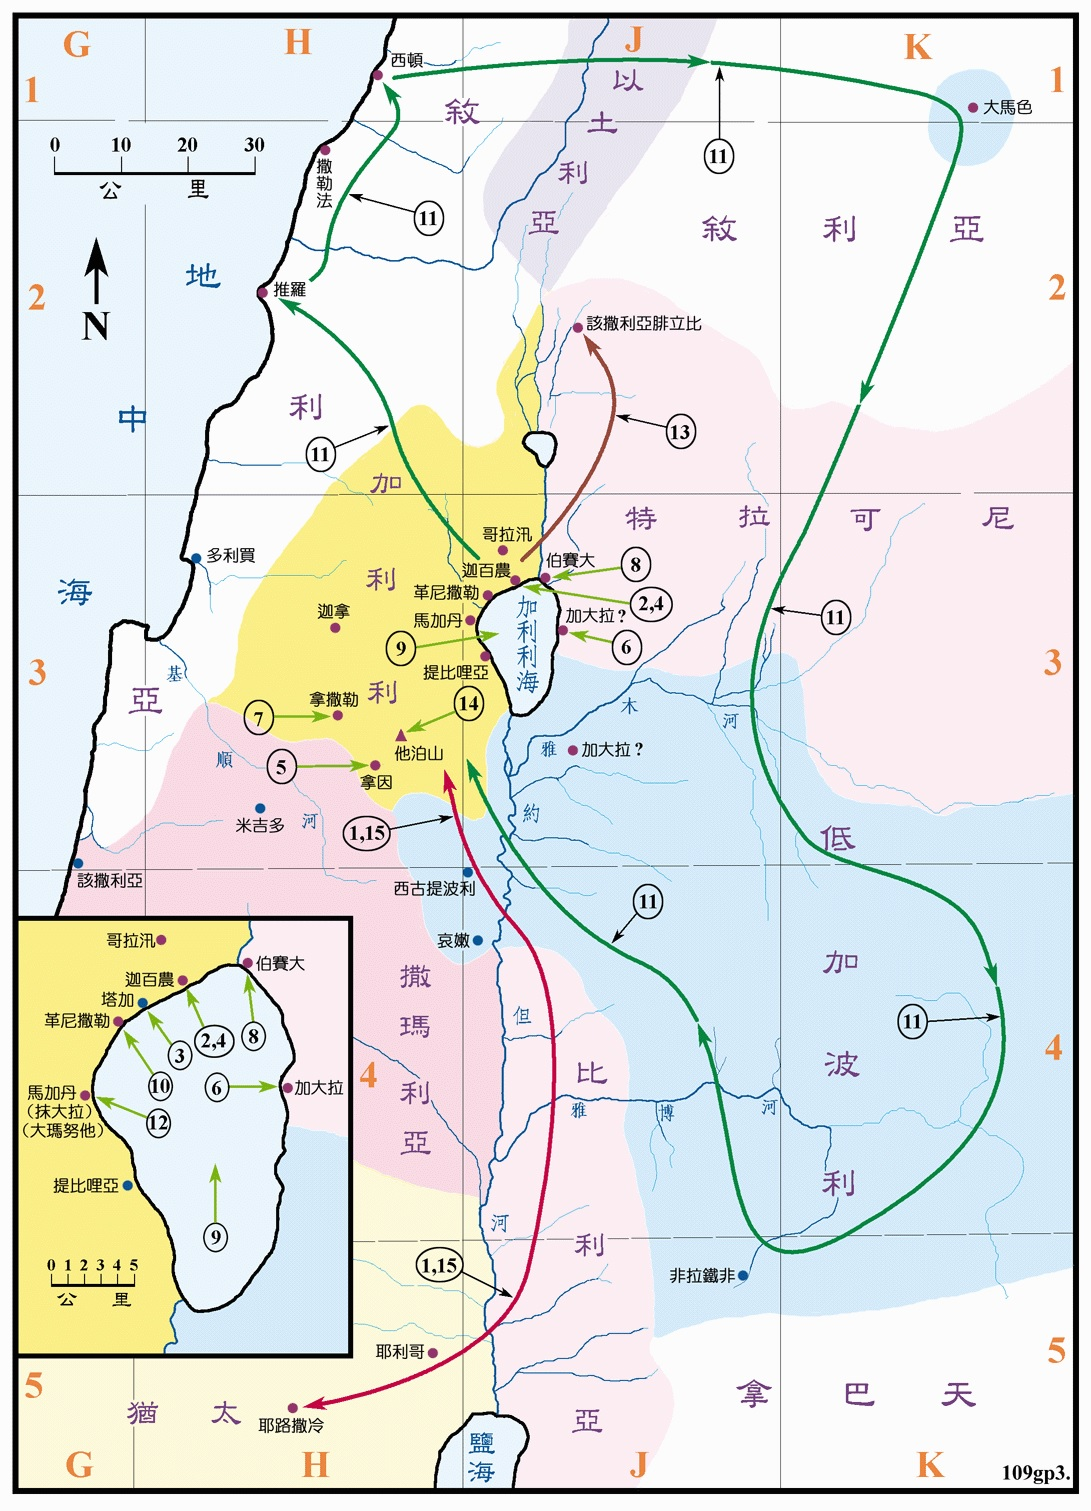
\includegraphics[width=170mm]{ZongJie/SiFuYin/figs/jesustripMinistry1}
 \caption{揀選门徒后的服事}
\end{figure}




%\subsection{设立使徒}
\subsubsection{拣选十二使徒后的初期培训}
\begin{table}[H]
\centering 
\begin{tabular}{p{13.07em}|p{8.43em}|p{5.285em}|p{5.57em}|p{5.285em}|p{4.855em}}
\toprule
\textbf{事 件} & \textbf{地 點} & \textbf{太} & \textbf{可} & \textbf{路} & \textbf{約} \\\midrule

為挑選十二門徒整夜禱告& 近迦百農山上  & \multicolumn{1}{r|}{} & & 6:12& \multicolumn{1}{r}{} \\ \midrule

\textcolor{blue}{設立十二使徒常和自己同在}& 近迦百農山上  & \multicolumn{1}{l|}{10:2-4} & 3:13-19 & 6:13-16 & \multicolumn{1}{r}{} \\ \midrule

百姓從猶太耶京推羅西頓來& \multicolumn{1}{l|}{海邊平地} & \multicolumn{1}{l|}{} & \multicolumn{1}{l|}{3:7-8} & 6:17& \multicolumn{1}{r}{} \\\midrule

醫病赶鬼,鬼认耶稣是神兒子& \multicolumn{1}{l|}{海邊平地} & \multicolumn{1}{l|}{} & \multicolumn{1}{l|}{3:9-12} & 6:18-19 & \multicolumn{1}{r}{} \\\midrule

登山教訓門徒論八福& 近迦百農山上  & 5:1-12& \multicolumn{1}{r|}{} & \multicolumn{1}{l|}{6:20-23} & \multicolumn{1}{r}{} \\    \midrule

富足飽足喜笑好人的四禍& 近迦百農山上&  & \multicolumn{1}{r|}{} & \multicolumn{1}{l|}{6:24-26} & \multicolumn{1}{r}{} \\    \midrule

門徒為鹽為光& 近迦百農山上& 5:13-16& \multicolumn{1}{r|}{} & \multicolumn{1}{r|}{} & \multicolumn{1}{r}{} \\    \midrule

成全律法和先知的道&\multicolumn{1}{l|}{\multirow{6}{*}{律法和先知}}& 5:17-20& \multicolumn{1}{r|}{} & \multicolumn{1}{r|}{} & \multicolumn{1}{r}{} \\   
\cmidrule{1-1}\cmidrule{3-6}{不可殺人愛仇敵}&& 5:21-26& \multicolumn{1}{r|}{} & \multicolumn{1}{r|}{} & \multicolumn{1}{r}{} \\   
\cmidrule{1-1}\cmidrule{3-6}{不可姦淫休妻}&   & 5:27-32& \multicolumn{1}{r|}{} & \multicolumn{1}{r|}{} & \multicolumn{1}{r}{} \\    
\cmidrule{1-1}\cmidrule{3-6}{不可背誓}&   & 5:33-37& \multicolumn{1}{r|}{} & \multicolumn{1}{r|}{} & \multicolumn{1}{r}{} \\   
\cmidrule{1-1}\cmidrule{3-6}{以眼還眼，以牙還牙}&   & 5:38-42& \multicolumn{1}{r|}{} & \multicolumn{1}{r|}{} & \multicolumn{1}{r}{} \\   
\cmidrule{1-1}\cmidrule{3-6}{愛鄰舍恨仇敵}&  & 5:43-48& \multicolumn{1}{r|}{} & \multicolumn{1}{l|}{6:27-38} & \multicolumn{1}{r}{} \\    \midrule

施捨&\multicolumn{1}{l|}{\multirow{3}{*}{行在暗中}}& 6:1-4& \multicolumn{1}{r|}{} & \multicolumn{1}{r|}{} & \multicolumn{1}{r}{} \\  
\cmidrule{1-1}\cmidrule{3-6}{禱告}&   & 6:5-15& \multicolumn{1}{r|}{} & \multicolumn{1}{r|}{} & \multicolumn{1}{r}{} \\  
\cmidrule{1-1}\cmidrule{3-6}{禁食}&  & 6:16-18& \multicolumn{1}{r|}{} & \multicolumn{1}{r|}{} & \multicolumn{1}{r}{} \\    \midrule

積攢財寶在天上& 近迦百農  & 6:19-21& \multicolumn{1}{r|}{} & \multicolumn{1}{r|}{} & \multicolumn{1}{r}{} \\    \midrule
眼睛就是身上的燈& 近迦百農  & 6:22-23 & \multicolumn{1}{r|}{} & \multicolumn{1}{r|}{} & \multicolumn{1}{r}{} \\    \midrule
不能侍奉兩個主& 近迦百農  & 6:24 & \multicolumn{1}{r|}{} & \multicolumn{1}{r|}{} & \multicolumn{1}{r}{} \\    \midrule
勿慮衣食不為明天憂慮& 近迦百農  & 6:25-34 & \multicolumn{1}{r|}{} & \multicolumn{1}{r|}{} & \multicolumn{1}{r}{} \\    \midrule

去掉自己眼中的梁木& 近迦百農  &  & \multicolumn{1}{r|}{} & \multicolumn{1}{l|}{6:39-42} & \multicolumn{1}{r}{} \\    \midrule

毋論斷人& 近迦百農  & 7:1-5 & \multicolumn{1}{r|}{} & \multicolumn{1}{r|}{} & \multicolumn{1}{r}{} \\    \midrule
不要把聖物給狗豬& 近迦百農  & 7:6 & \multicolumn{1}{r|}{} & \multicolumn{1}{r|}{} & \multicolumn{1}{r}{} \\    \midrule
祈求尋找叩門& 近迦百農  & 7:7-12 & \multicolumn{1}{r|}{} & \multicolumn{1}{r|}{} & \multicolumn{1}{r}{} \\    \midrule
兩條門路& 近迦百農  & 7:13-14 & \multicolumn{1}{r|}{} & \multicolumn{1}{r|}{} & \multicolumn{1}{r}{} \\    \midrule
兩種果樹& 近迦百農  & 7:15-23 & \multicolumn{1}{r|}{} & \multicolumn{1}{l|}{6:43-45} & \multicolumn{1}{r}{} \\    \midrule
兩等根基& 近迦百農  & 7:24-27 & \multicolumn{1}{r|}{} & \multicolumn{1}{l|}{6:46-49} & \multicolumn{1}{r}{} \\    \midrule
耶穌的教訓像有權柄的人& 近迦百農  & 7:28-29& \multicolumn{1}{r|}{} & \multicolumn{1}{r|}{} & \multicolumn{1}{r}{} \\    \midrule

耶穌醫百夫長的僕人 & 迦百農   & 8:5-13 & \multicolumn{1}{r|}{} & 7:1-10 & \multicolumn{1}{r}{} \\\midrule

耶穌使寡婦兒子複生 & 拿因    & \multicolumn{1}{r|}{} & \multicolumn{1}{r|}{} & 7:11-17 & \multicolumn{1}{r}{} \\ \midrule

\textcolor{blue}{約翰在監差兩門徒問主该等谁} & 加利利   & 11:2-6& \multicolumn{1}{r|}{} & 7:18-23& \multicolumn{1}{r}{} \\ \midrule

\textcolor{blue}{差人走后主對眾人讚施洗約翰}& 加利利   & 11:7-15& \multicolumn{1}{r|}{} & 7:24-29& \multicolumn{1}{r}{} \\ \midrule

警法利賽人律法師辨别世代& 加利利   & 11:16-19& \multicolumn{1}{r|}{} & 7:30-35& \multicolumn{1}{r}{} \\ \midrule

耶穌坐席时有罪女人膏主 & 迦百農   & \multicolumn{1}{r|}{} & \multicolumn{1}{r|}{} & 7:36-50 & \multicolumn{1}{r}{} \\\midrule

耶穌周游传道的同工团队 & 加利利   & \multicolumn{1}{r|}{} & \multicolumn{1}{r|}{} & 8:1-3 & \multicolumn{1}{r}{} \\ \midrule

\end{tabular}%
\end{table}%

%\subsubsection{拣选十二使徒后的初期培训}
\begin{table}[H]
\centering 
\begin{tabular}{p{13.07em}|p{8.43em}|p{5.285em}|p{5.57em}|p{5.285em}|p{4.855em}}
\toprule
\textbf{事 件} & \textbf{地 點} & \textbf{太} & \textbf{可} & \textbf{路} & \textbf{約} \\\midrule

坐船上對眾人講天國結實百倍& 加利利迦百農海邊& \multicolumn{1}{l|}{13:1-9} & \multicolumn{1}{l|}{4:1-9} & 8:4-8 & \multicolumn{1}{r}{} \\ \midrule
對門徒解释用比喻的原因& 加利利迦百農海邊& \multicolumn{1}{l|}{13:10-16} & \multicolumn{1}{l|}{4:10-12} & 8:9-10 & \multicolumn{1}{r}{} \\ \midrule
對門徒解明撒種的比喻& 加利利迦百農海邊& \multicolumn{1}{l|}{13:17-23} & \multicolumn{1}{l|}{4:13-20} & 8:11-15 & \multicolumn{1}{r}{} \\ \midrule

置燈于臺上喻掩藏的事必顯明& 加利利迦百農海邊& \multicolumn{1}{l|}{} & \multicolumn{1}{l|}{4:21-23} & 8:16-17 & \multicolumn{1}{r}{} \\ \midrule

用量器量給人必得回报且多得& 加利利迦百農海邊& \multicolumn{1}{l|}{} & \multicolumn{1}{l|}{4:24} & & \multicolumn{1}{r}{} \\ \midrule

凡有的還要加給他& 加利利迦百農海邊& \multicolumn{1}{l|}{} & \multicolumn{1}{l|}{4:25} & 8:18& \multicolumn{1}{r}{} \\ \midrule

收割時候分开田裡麥子稗子& 加利利迦百農海邊& \multicolumn{1}{l|}{13:24-30} & \multicolumn{1}{l|}{4:26-29} & & \multicolumn{1}{r}{} \\ \midrule

芥菜種宿天上飛鳥的比喻& 加利利迦百農海邊& \multicolumn{1}{l|}{13:31-32} & \multicolumn{1}{l|}{4:30-32} & & \multicolumn{1}{r}{} \\ \midrule

對眾人用比喻给門徒解明比喻& 加利利迦百農海邊& \multicolumn{1}{l|}{} & \multicolumn{1}{l|}{4:33-34} & & \multicolumn{1}{r}{} \\ \midrule

婦人麵酵的比喻& 加利利迦百農海邊& \multicolumn{1}{l|}{13:33} & \multicolumn{1}{l|}{} & & \multicolumn{1}{r}{} \\ \midrule
用比喻對人說話應驗先知预言& 加利利迦百農海邊& \multicolumn{1}{l|}{13:34-35} & \multicolumn{1}{l|}{} & & \multicolumn{1}{r}{} \\ \midrule
對門徒解明稗子的比喻& 加利利迦百農房子& \multicolumn{1}{l|}{13:36-43} & \multicolumn{1}{l|}{} & & \multicolumn{1}{r}{} \\ \midrule
變賣一切買藏寶之地& 加利利迦百農海邊& \multicolumn{1}{l|}{13:44}& \multicolumn{1}{l|}{} && \multicolumn{1}{r}{} \\ \midrule
買賣人變賣一切買好珠子& 加利利迦百農海邊& \multicolumn{1}{l|}{13:45-46} & \multicolumn{1}{l|}{} &  & \multicolumn{1}{r}{} \\ \midrule

以天國網撒喻世界末了& 加利利迦百農海邊& \multicolumn{1}{l|}{13:47-50} & \multicolumn{1}{l|}{} && \multicolumn{1}{r}{} \\ \midrule
家主庫裡拿出的新舊東西& 加利利迦百農海邊& \multicolumn{1}{l|}{13:51-52} & \multicolumn{1}{l|}{} & & \multicolumn{1}{r}{} \\ \midrule
%& 加利利迦百農海邊& \multicolumn{1}{l|}{13:} & \multicolumn{1}{l|}{4:} & 8: & \multicolumn{1}{r}{} \\ \midrule
%耶穌對法利賽人的講論？？ & 加利利   & 12:22-45 & 3:22-30 & 11:14-36 & \multicolumn{1}{r}{} \\ \midrule

耶穌論信者皆为親屬 & 加利利   & 12:46-50 & 3:31-35 & 8:19-21 & \multicolumn{1}{r}{} \\ \midrule

耶穌船尾睡覺，平靜風浪 & 加利利海  & 8:23-27 & 4:35-41 & 8:22-25 & \multicolumn{1}{r}{} \\
    \midrule
耶穌趕逐諸鬼入豬群 & 格拉森/加大拉& 8:28-34 & 5:1-20 & 8:26-39 & \multicolumn{1}{r}{} \\
    \midrule
醫血漏妇人/管会堂女儿復活& 迦百農   & 9:18-26 & 5:21-43 & 8:40-56 & \multicolumn{1}{r}{} \\
    \midrule
%耶穌使管会堂的女儿復活 & 迦百農   & 9:18-26 & 5:21-43 & 8:40-56 & \multicolumn{1}{r}{} \\   \midrule
摸兩個瞎子的眼睛醫治他們& 迦百農房子裡& 9:27-31 & \multicolumn{1}{r|}{} & \multicolumn{1}{r|}{} & \multicolumn{1}{r}{} \\ \midrule
耶穌使鬼附的一個啞吧說話 & 迦百農出房子時 & 9:32-33& \multicolumn{1}{r|}{} & \multicolumn{1}{r|}{} & \multicolumn{1}{r}{} \\\midrule
法利賽人說：他靠鬼王趕鬼& 迦百農出房子時 & 9:34 & \multicolumn{1}{r|}{} & \multicolumn{1}{r|}{} & \multicolumn{1}{r}{} \\\midrule
安息日在會堂裡教訓再次被拒&拿撒勒&13:53-58& \multicolumn{1}{l|}{6:1-6} & \multicolumn{1}{r|}{} & \multicolumn{1}{r}{} \\\midrule
耶穌往各城去傳道 & 加利利   & \multicolumn{1}{l|}{9:35} & 6:6下  & \multicolumn{1}{r|}{} & \multicolumn{1}{r}{} \\ \midrule

%\textbf{耶穌差遣十二使徒傳道} & 加利利   & 9:36-11:1 & 6:7-13 & 9:1-6 & \multicolumn{1}{r}{} \\ \midrule
\textbf{憐憫眾人,莊稼多,工人少} & 加利利   & 9:36-38&  &  & \multicolumn{1}{r}{} \\ \midrule
\end{tabular}%
\end{table}%

\subsubsection{差遣十二使徒传道的培训}
\begin{table}[H]
\centering 
\begin{tabular}{p{17.07em}|p{8.43em}|p{5.285em}|p{5em}|p{4.285em}|p{1.855em}}\toprule
\textbf{事 件} & \textbf{地 點} & \textbf{太} & \textbf{可} & \textbf{路} & \textbf{約} \\\midrule

\textcolor{blue}{給十二使徒權柄兩兩出去傳道} & 加利利   & 10:1& 6:7& 9:1-2& \multicolumn{1}{r}{} \\ \midrule
\textbf{往以色列傳天國近了} &地点/内容& 10:5-6 &  &  & \multicolumn{1}{r}{} \\ \midrule
%\textbf{内容:天國近了} & 加利利   & 10:7 & & & \multicolumn{1}{r}{} \\ \midrule
\textbf{免费醫病潔淨痲瘋趕鬼} &方法& 10:8& & & \multicolumn{1}{r}{} \\ \midrule
\textbf{不帶食物錢靠做工得食} & 原则& 10:9-10& 6:8-9& 9:3 & \multicolumn{1}{r}{} \\ \midrule
\textbf{進谁家就住在那裡/如同羊進入狼群} &住宿/危险 & 10:11-15& 6:10-11& 9:4-5 & \multicolumn{1}{r}{} \\ \midrule
%\textbf{如同羊進入狼群} &危险& 10:16-20& & & \multicolumn{1}{r}{} \\ \midrule

\textbf{忍耐到底必然得救/不要懼怕} &态度& 10:21-23&& & \multicolumn{1}{r}{} \\ \midrule
%\textbf{态度2：不要懼怕} & 加利利   &10:24-33& && \multicolumn{1}{r}{} \\ \midrule
\textbf{背著他的十字架/接待義人得義的賞賜} &代价/賞賜&10:34-39&  && \multicolumn{1}{r}{} \\ \midrule
\end{tabular}%
\end{table}%

\subsubsection{施洗约翰被杀后的工作}
\begin{table}[H]\centering 
\begin{tabular}{p{13.07em}|p{8.43em}|p{5.285em}|p{5.57em}|p{5.285em}|p{4.855em}}
\toprule
\textbf{事 件} & \textbf{地 點} & \textbf{太} & \textbf{可} & \textbf{路} & \textbf{約} \\\midrule
門徒就出去傳道叫人悔改& 加利利   &&6:12-13& 9:6& \multicolumn{1}{r}{} \\ \midrule

主吩咐完就往各城傳道教訓人& &11:1&&& \multicolumn{1}{r}{} \\ \midrule


\textcolor{red}{複記施洗約翰被殺經過} & 馬格路斯堡 & 14:6-12 & 6:21-29 & \multicolumn{1}{r|}{} & \multicolumn{1}{r}{} \\ \midrule

众人和希律猜测耶穌身份& 加利利   &14:1-2& 6:14-16 & 9:7-9 & \multicolumn{1}{r}{} \\ \midrule

%& 14:1-2 & 6:14-16 & 9:7-9 & \multicolumn{1}{r}{} \\ \midrule

使徒传道回来聚集到耶穌前& 伯賽大旷野&  & 6:30-32& 9:10 &  \\
   \midrule     


%\multicolumn{1}{p{12.5em}|}{畢士大池醫38年瘫子} & \multicolumn{1}{l|}{\multirow{4}{*}{耶路撒冷,可能是早期}}&       &       &       & 5:1-15\\
%\cmidrule{1-1}\cmidrule{3-6}猶太人逼迫主犯安息日想杀他&       &       &       &       & 5:16-18\\
%\cmidrule{1-1}\cmidrule{3-6}子遵父命，父給子審判權 &       &       &       &       & 5:19-30 \\
%\cmidrule{1-1}\cmidrule{3-6}見證:約翰/所行/父/聖經/摩西&       &       &       &       & 5:31-47\\ \midrule

逾越節前使五千人吃飽 & 伯賽大旷野& 14:13-21 & 6:33-44 & 9:11-17 & 6:1-14 \\
   \midrule  

門徒在船上,耶穌在海面行走 & 加利利海  & 14:22-27& 6:45-52 &       & \multicolumn{1}{p{4.855em}}{6:15-21} \\\midrule

彼得在海面行走因害怕而下沉& 加利利海  & 14:28-33 & &       & \multicolumn{1}{p{4.855em}}{} \\\midrule


論信神所差來的就是做神的工& 迦百農海邊& \multicolumn{1}{r|}{} & \multicolumn{1}{r|}{} &       & \multicolumn{1}{p{4.855em}}{6:22-29} \\\midrule
耶穌論生命的糧 & 迦百農會堂   & \multicolumn{1}{r|}{} & \multicolumn{1}{r|}{} &       & \multicolumn{1}{p{4.855em}}{6:30-40} \\\midrule
對猶太人論吃人子肉喝人子血& 迦百農會堂   & \multicolumn{1}{r|}{} & \multicolumn{1}{r|}{} &       & \multicolumn{1}{p{4.855em}}{6:41-59} \\\midrule

對門徒論話就是靈就是生命& 迦百農& \multicolumn{1}{r|}{} & \multicolumn{1}{r|}{} &       & \multicolumn{1}{p{4.855em}}{6:60-66} \\\midrule
彼得确认從主，启示猶大賣主& 迦百農& \multicolumn{1}{r|}{} & \multicolumn{1}{r|}{} &       & \multicolumn{1}{p{4.855em}}{6:67-71} \\\midrule


耶穌下船后在革尼撒勒醫病 & 革尼撒勒伯賽大 & 14:34-36 & 6:53-56 &       &  \\ \midrule

耶京法利賽人文士责門徒俗手&  & 15:1-2& 7:1-5&       &  \\\midrule
主责应验以赛亚"嘴唇敬主"&  & 15:7-9& 7:6-7 &       &  \\\midrule
主责其廢神誡命守人遺傳&  & 15:3-6& 7:8-13 &       &  \\\midrule

對眾人說出口的乃能汙穢人&  & 15:10-11 & 7:14-16&       &  \\\midrule
門徒告主說法利賽人不服&  & 15:12&  &       &  \\\midrule
非天父栽種必拔出,瞎子領路&  & 15:13-14 &  &       &  \\\midrule
對彼得解释出口的汙穢人& 離開眾人進了屋子& 15:15-20& 7:17-23&       &  \\\midrule

耶穌醫迦南婦人的女兒 & \multicolumn{1}{p{7.93em}|}{推羅西頓進一家} & \multicolumn{1}{p{5.285em}|}{15:21-28} & \multicolumn{1}{p{5.57em}|}{7:24-30} & \multicolumn{1}{r|}{} &  \\\midrule
用指頭吐唾醫耳聾舌者結& \multicolumn{1}{p{7.93em}|}{加利利海} & \multicolumn{1}{p{5.285em}|}{} & \multicolumn{1}{p{5.57em}|}{7:31-37} & \multicolumn{1}{r|}{} &  \\\midrule
耶穌醫聾啞其他病人 & \multicolumn{1}{p{7.93em}|}{加利利海山上} & \multicolumn{1}{p{5.285em}|}{15:29-31} & \multicolumn{1}{p{5.57em}|}{} & \multicolumn{1}{r|}{} &  \\\midrule
\multicolumn{1}{l|}{耶穌使四千人吃飽} & \multicolumn{1}{p{7.93em}|}{低加波利野地} & \multicolumn{1}{p{5.285em}|}{15:32-38} & \multicolumn{1}{p{5.57em}|}{8:1-9} & \multicolumn{1}{r|}{} &  \\ \midrule
同門徒上船到大瑪努他境內& \multicolumn{1}{p{7.93em}|}{馬加丹/大瑪努他} & \multicolumn{1}{p{5.285em}|}{15:39} & \multicolumn{1}{p{5.57em}|}{8:10} & \multicolumn{1}{r|}{} &  \\     \bottomrule

責法利賽撒都該人求天上神迹& \multicolumn{1}{p{7.93em}|}{馬加丹/大瑪努他} & \multicolumn{1}{p{5.285em}|}{16:1-4} & \multicolumn{1}{p{5.57em}|}{8:11-13} & \multicolumn{1}{r|}{} &  \\ \midrule

警告門徒防法利賽人和撒都該/希律的酵(教訓)& \multicolumn{1}{p{7.93em}|}{加利利海船上} & \multicolumn{1}{p{5.285em}|}{16:5-12} & \multicolumn{1}{p{5.57em}|}{8:14-21} & \multicolumn{1}{r|}{} &  \\ \midrule

耶穌吐唾沫又按手使瞎子看見 & \multicolumn{1}{p{7.93em}|}{伯賽大村外} &       & \multicolumn{1}{p{5.57em}|}{8:22-26} &\multicolumn{1}{r|}{} &  \\ \midrule

\end{tabular}%
\caption{到第三個逾越節}
\label{tab:addlabel}%
\end{table}%

\subsection{启示自己受死并复活}
\begin{table}[H] \centering 
\begin{tabular}{p{13.07em}|l|l|l|p{5.285em}|r}\toprule
\textbf{事 件} & \multicolumn{1}{p{7.93em}|}{\textbf{地 點}} & \multicolumn{1}{p{5.285em}|}{\textbf{馬太福音}} & \multicolumn{1}{p{5.57em}|}{\textbf{馬可福音}} & \textbf{路加福音} & \multicolumn{1}{p{4.855em}}{\textbf{約翰福音}} \\\midrule

途中主問門徒:人說人子是誰& \multicolumn{1}{p{7.93em}|}{該撒利亞腓立比} & \multicolumn{1}{p{5.285em}|}{16:13-14} & \multicolumn{1}{p{5.57em}|}{8:27-28} & 9:18-19&  \\ \midrule

彼得認耶穌爲神的兒子 & \multicolumn{1}{p{7.93em}|}{該撒利亞腓立比} & \multicolumn{1}{p{5.285em}|}{16:15-16} & \multicolumn{1}{p{5.57em}|}{8:29-30} & 9:20-21&  \\ \midrule

对彼得论把教會建造在磐石上& \multicolumn{1}{p{7.93em}|}{該撒利亞腓立比} & \multicolumn{1}{p{5.285em}|}{16:17-18a} & \multicolumn{1}{p{5.57em}|}{} &  &  \\ \midrule

天國鑰匙/捆綁釋放權柄& \multicolumn{1}{p{7.93em}|}{該撒利亞腓立比} & \multicolumn{1}{p{5.285em}|}{16:18b-20} & \multicolumn{1}{p{5.57em}|}{} &  &  \\ \midrule

\textcolor{red}{首次}提說在耶路撒冷被殺復活& \multicolumn{1}{p{7.93em}|}{該撒利亞腓立比} & \multicolumn{1}{p{5.285em}|}{16:21} & \multicolumn{1}{p{5.57em}|}{8:31} & 9:22&  \\ \midrule

彼得拦主被责撒旦不體貼神意& \multicolumn{1}{p{7.93em}|}{該撒利亞腓立比} & \multicolumn{1}{p{5.285em}|}{16:22-23} & \multicolumn{1}{p{5.57em}|}{8:32-33} &&  \\ \midrule

教導門徒背十字架跟從主& \multicolumn{1}{p{7.93em}|}{該撒利亞腓立比} & \multicolumn{1}{p{5.285em}|}{16:24-26} & \multicolumn{1}{p{5.57em}|}{8:34-37} & 9:23-25&  \\ \midrule


人子在榮耀降臨時不认背主者& \multicolumn{1}{p{7.93em}|}{該撒利亞腓立比} & \multicolumn{1}{p{5.285em}|}{16:27} & \multicolumn{1}{p{5.57em}|}{8:38} & 9:26&  \\ \midrule

预言有人在沒死前見主荣神國& \multicolumn{1}{p{7.93em}|}{該撒利亞腓立比} & \multicolumn{1}{p{5.285em}|}{16:28} & \multicolumn{1}{p{5.57em}|}{9:1} & 9:27 &  \\ \midrule


6天后彼得雅各約翰见主變像& \multicolumn{1}{p{7.93em}|}{腓立比黑門山上} & \multicolumn{1}{p{5.285em}|}{17:1-8} & \multicolumn{1}{p{5.57em}|}{9:2-8} & 9:28-36 &  \\ \midrule
 
戒门徒死裡復活前勿讲此事& \multicolumn{1}{p{7.93em}|}{下腓立比黑門山} & \multicolumn{1}{p{5.285em}|}{17:9} & \multicolumn{1}{p{5.57em}|}{9:9-10} &  &  \\ \midrule
  
以約翰譬以利亞/\textcolor{red}{人子要受害}& \multicolumn{1}{p{7.93em}|}{下腓立比黑門山} & \multicolumn{1}{p{5.285em}|}{17:10-13} & \multicolumn{1}{p{5.57em}|}{9:11-13} &  &  \\ \midrule


耶穌醫治癲癇的孩子 & \multicolumn{1}{p{7.93em}|}{腓立比黑門山下} & \multicolumn{1}{p{5.285em}|}{17:14-18} & \multicolumn{1}{p{5.57em}|}{9:14-27} & 9:37-43a &  \\\midrule

門徒暗問赶鬼失败的原因& \multicolumn{1}{p{7.93em}|}{黑門山下屋子里} & \multicolumn{1}{p{5.285em}|}{17:19} & \multicolumn{1}{p{5.57em}|}{9:28} & &  \\\midrule
告門徒有信心可移山& \multicolumn{1}{p{7.93em}|}{黑門山下屋子里} & \multicolumn{1}{p{5.285em}|}{17:20} & \multicolumn{1}{p{5.57em}|}{} & &  \\\midrule
告門徒信心小时禁食禱告赶鬼& \multicolumn{1}{p{7.93em}|}{黑門山下屋子里} & \multicolumn{1}{p{5.285em}|}{17:21} & \multicolumn{1}{p{5.57em}|}{9:29} & &  \\\midrule

\textbf{耶穌對門徒\textcolor{red}{三論}受害的事} & \multicolumn{1}{p{7.93em}|}{住在加利利} & \multicolumn{1}{p{5.285em}|}{17:22-23} & \multicolumn{1}{p{5.57em}|}{9:30-32} & 9:43b-45 &  \\ \midrule

在路上彼此爭論誰為大& \multicolumn{1}{p{7.93em}|}{去迦百農路上} & \multicolumn{1}{p{5.285em}|}{} & \multicolumn{1}{p{5.57em}|}{9:33-34} & 9:46&  \\ \midrule

門徒問「天國裡誰是最大的」& \multicolumn{1}{p{7.93em}|}{迦百農在屋裡} & \multicolumn{1}{p{5.285em}|}{18:1} & \multicolumn{1}{p{5.57em}|}{} & &  \\ \midrule

願意做首的必做眾人的用人& \multicolumn{1}{p{7.93em}|}{迦百農} & \multicolumn{1}{p{5.285em}|}{} & \multicolumn{1}{p{5.57em}|}{9:35} &  &  \\ \midrule


不成小孩子不得進天國& \multicolumn{1}{p{7.93em}|}{迦百農在屋裡} & \multicolumn{1}{p{5.285em}|}{18:2-3} & \multicolumn{1}{p{5.57em}|}{10:15} & &  \\ \midrule

謙卑像這小孩子是最大的& \multicolumn{1}{p{7.93em}|}{迦百農在屋裡} & \multicolumn{1}{p{5.285em}|}{18:4} & \multicolumn{1}{p{5.57em}|}{} & &  \\ \midrule

%門徒爭大,教導最小的為大& \multicolumn{1}{p{7.93em}|}{迦百農} & \multicolumn{1}{p{5.285em}|}{18:1-6} & \multicolumn{1}{p{5.57em}|}{9:33-37} & 9:46-48 &  \\ \midrule

接待小孩就是接待主& \multicolumn{1}{p{7.93em}|}{迦百農} & \multicolumn{1}{p{5.285em}|}{18:5} & \multicolumn{1}{p{5.57em}|}{9:36-37} & 9:47-48a &  \\ \midrule

你們中間最小的他便為大& \multicolumn{1}{p{7.93em}|}{迦百農} & \multicolumn{1}{p{5.285em}|}{} & \multicolumn{1}{p{5.57em}|}{9:36-37} & 9:48b &  \\ \midrule

彼得自魚口中得銀納稅 & \multicolumn{1}{p{7.93em}|}{迦百農} & \multicolumn{1}{p{5.285em}|}{17:24-27} &       & \multicolumn{1}{r|}{} &  \\  \midrule

教導約翰不要禁止人趕鬼& \multicolumn{1}{p{7.93em}|}{迦百農} &&\multicolumn{1}{p{5.57em}|}{9:38-40} & 9:49-50 &  \\\midrule

因你們屬基督給水喝必得賞賜& \multicolumn{1}{p{7.93em}|}{迦百農} &&\multicolumn{1}{p{5.57em}|}{9:41} &  &  \\\midrule

%使信主小子跌倒的不如去死& \multicolumn{1}{p{7.93em}|}{迦百農} & \multicolumn{1}{p{5.285em}|}{18:6-7} & \multicolumn{1}{p{5.57em}|}{9:42} & &  \\ \midrule

残肢入永生强如全人进地狱& \multicolumn{1}{p{7.93em}|}{迦百農?} &\multicolumn{1}{p{5.285em}|}{18:8-9}&9:43-47&  &  \\\midrule
地狱蟲不死火不滅鹽醃各人& \multicolumn{1}{p{7.93em}|}{迦百農?} &\multicolumn{1}{p{5.285em}|}{}&9:48-49&  &  \\\midrule
裡頭應當有鹽彼此和睦& \multicolumn{1}{p{7.93em}|}{迦百農?} &\multicolumn{1}{p{5.285em}|}{}&9:50&  &  \\\midrule

小子的使者在天上常見天父& \multicolumn{1}{p{7.93em}|}{迦百農?} &\multicolumn{1}{p{5.285em}|}{18:10}&9:42-50&  &  \\\midrule


被弟兄得罪时的处理方法& \multicolumn{1}{p{7.93em}|}{迦百農?} &\multicolumn{1}{p{5.285em}|}{18:15-17}&&  &  \\\midrule

在地上捆綁和釋放的权柄& \multicolumn{1}{p{7.93em}|}{迦百農?} &\multicolumn{1}{p{5.285em}|}{18:18}&&  &  \\\midrule
两人同心求就有主同在& \multicolumn{1}{p{7.93em}|}{迦百農?} &\multicolumn{1}{p{5.285em}|}{18:19-20}&&  &  \\\midrule
對彼得说饒恕七十個七次& \multicolumn{1}{p{7.93em}|}{迦百農?} &\multicolumn{1}{p{5.285em}|}{18:21-22}&&  &  \\\midrule
欠十兩銀子的仆人& \multicolumn{1}{p{7.93em}|}{迦百農?} &\multicolumn{1}{p{5.285em}|}{18:23-35}&&  &  \\\midrule
\end{tabular}
\end{table}%




\subsubsection{耶穌在住棚節時的講論}
\begin{table}[H]\centering 
\begin{tabular}{p{13.07em}|l|l|l|p{5.285em}|r}\toprule
\textbf{事 件} & \multicolumn{1}{p{7.93em}|}{\textbf{地 點}} & \multicolumn{1}{p{5.285em}|}{\textbf{馬太福音}} & \multicolumn{1}{p{5.57em}|}{\textbf{馬可福音}} & \textbf{路加福音} & \multicolumn{1}{p{4.855em}}{\textbf{約翰福音}} \\\midrule 

猶太人想要殺他& \multicolumn{1}{p{7.93em}|}{加利利} & \multicolumn{1}{p{5.285em}|}{} & \multicolumn{1}{p{5.57em}|}{} &  &\multicolumn{1}{l}{7:1}  \\ \midrule

\textbf{住棚節時耶穌弟兄不信耶穌} & \multicolumn{1}{p{7.93em}|}{加利利} &       &       & \multicolumn{1}{r|}{} & \multicolumn{1}{p{4.855em}}{7:2-10} \\\midrule

對跟随文士論人子无枕之地& \multicolumn{1}{p{7.93em}|}{迦百農渡口} & \multicolumn{1}{p{5.285em}|}{8:18-20} &       & 9:57-58&  \\ \midrule

對葬父之人論任死人葬其死人& \multicolumn{1}{p{7.93em}|}{迦百農渡口} & \multicolumn{1}{p{5.285em}|}{8:21-22} &       & 9:59-60&  \\ \midrule

對人論扶犁向後看不配進神國& \multicolumn{1}{p{7.93em}|}{迦百農渡口} & \multicolumn{1}{p{5.285em}|}{} &       & 9:61-62 &  \\ \midrule

去耶京时瑪利亞人不接待主& \multicolumn{1}{p{7.93em}|}{\textcolor{red}{耶京過撒瑪利亞}} &  &  & 9:51-56 &  \\\midrule

\textbf{猶太人找耶穌稀奇其教訓} & \multicolumn{1}{p{7.93em}|}{住棚節耶路撒冷} &       &       & \multicolumn{1}{r|}{} & \multicolumn{1}{p{4.855em}}{7:11-15} \\\midrule

\textbf{耶穌求那差他來者的榮耀} & \multicolumn{1}{p{7.93em}|}{住棚節耶路撒冷} &       &       & \multicolumn{1}{r|}{} & \multicolumn{1}{p{4.855em}}{7:16-18} \\\midrule

\textbf{向眾人論安息日治病} & \multicolumn{1}{p{7.93em}|}{住棚節耶路撒冷} &       &       & \multicolumn{1}{r|}{} & \multicolumn{1}{p{4.855em}}{7:19-24} \\\midrule

\textbf{向眾人論父差子} & \multicolumn{1}{p{7.93em}|}{住棚節耶路撒冷} &       &       & \multicolumn{1}{r|}{} & \multicolumn{1}{p{4.855em}}{7:25-29} \\\midrule

\textbf{打發差役捉拿耶穌} & \multicolumn{1}{p{7.93em}|}{住棚節耶路撒冷} &       &       & \multicolumn{1}{r|}{} & \multicolumn{1}{p{4.855em}}{7:30-36} \\\midrule

\textbf{向眾人論腹中的活水江河} & \multicolumn{1}{p{7.93em}|}{住棚節耶路撒冷} &       &       & \multicolumn{1}{r|}{} & \multicolumn{1}{p{4.855em}}{7:37-44} \\\midrule
\textbf{法利賽人责差役尼哥迪慕} & \multicolumn{1}{p{7.93em}|}{住棚節耶路撒冷} &       &       & \multicolumn{1}{r|}{} & \multicolumn{1}{p{4.855em}}{7:45-52} \\\midrule
    耶穌赦免犯罪的婦人 & \multicolumn{1}{p{7.93em}|}{住棚節耶路撒冷} &       &       & \multicolumn{1}{r|}{} & \multicolumn{1}{p{4.855em}}{8:1-11} \\ \midrule
    耶穌論光與自由 & \multicolumn{1}{p{7.93em}|}{住棚節耶路撒冷} &       &       & \multicolumn{1}{r|}{} & \multicolumn{1}{p{4.855em}}{8:12-59} \\\midrule
    耶穌醫生來瞎眼者 & \multicolumn{1}{p{7.93em}|}{住棚節耶路撒冷} &       &       & \multicolumn{1}{r|}{} & \multicolumn{1}{p{4.855em}}{9:1-41} \\ \midrule
    耶穌論羊的門好牧人 & \multicolumn{1}{p{7.93em}|}{住棚節耶路撒冷} &       &       & \multicolumn{1}{r|}{} & \multicolumn{1}{p{4.855em}}{10:1-21} \\\midrule
   
\end{tabular}%
\end{table}%

\subsubsection{差遣七十人兩兩传道}

\begin{table}[H] \centering 
\begin{tabular}{p{13.07em}|l|l|l|p{5.285em}|r} \toprule
\textbf{事 件} & \multicolumn{1}{p{7.93em}|}{\textbf{地 點}} & \multicolumn{1}{p{5.285em}|}{\textbf{馬太福音}} & \multicolumn{1}{p{5.57em}|}{\textbf{馬可福音}} & \textbf{路加福音} & \multicolumn{1}{p{4.855em}}{\textbf{約翰福音}} \\\midrule 

\textcolor{red}{差遣七十人兩兩在主前走}& \multicolumn{1}{p{7.93em}|}{去耶京途中} & \multicolumn{1}{p{5.285em}|}{} &       & 10:1&  \\\midrule

當求莊稼主打發工人收莊稼& \multicolumn{1}{p{7.93em}|}{} & \multicolumn{1}{p{5.285em}|}{} &       & 10:2&  \\\midrule

如同羊羔進入狼群& \multicolumn{1}{p{7.93em}|}{去耶京途中} & \multicolumn{1}{p{5.285em}|}{} &       & 10:3&  \\\midrule
不帶錢囊口袋鞋& \multicolumn{1}{p{7.93em}|}{去耶京途中？} & \multicolumn{1}{p{5.285em}|}{} &       & 10:4&  \\\midrule
为所住的家求的平安& \multicolumn{1}{p{7.93em}|}{} & \multicolumn{1}{p{5.285em}|}{} &       & 10:5-6&  \\\midrule

靠传福音糊口& \multicolumn{1}{p{7.93em}|}{} & \multicolumn{1}{p{5.285em}|}{} &       & 10:7-8&  \\\midrule
内容：神的國臨近你們了& \multicolumn{1}{p{7.93em}|}{} & \multicolumn{1}{p{5.285em}|}{} &       & 10:9-11&  \\\midrule
哥拉汛伯賽大迦百農之禍& \multicolumn{1}{p{7.93em}|}{} & \multicolumn{1}{p{5.285em}|}{11:20-24} &       & 10:12-15&  \\\midrule
對門徒說聽你們的就是聽我& \multicolumn{1}{p{7.93em}|}{} & \multicolumn{1}{p{5.285em}|}{} &       & 10:16&  \\\midrule

對七十人說撒旦從天上墜落& \multicolumn{1}{p{7.93em}|}{} & \multicolumn{1}{p{5.285em}|}{} &       & 10:17-19 &  \\\midrule
要因名記錄在天上歡喜& \multicolumn{1}{p{7.93em}|}{} & \multicolumn{1}{p{5.285em}|}{} &       & 10:20 &  \\\midrule

耶穌被聖靈感動歡樂頌神 & \multicolumn{1}{p{7.93em}|}{去耶京途中？} & \multicolumn{1}{p{5.285em}|}{11:25-27} &       & 10:21-22 &  \\ \midrule
勞苦擔重擔者得安息享安息& \multicolumn{1}{p{7.93em}|}{去耶京途中？} & \multicolumn{1}{p{5.285em}|}{11:28-30} &       &  &  \\ \midrule
對門徒說看見你們看見的有福& \multicolumn{1}{p{7.93em}|}{去耶京途中？} & \multicolumn{1}{p{5.285em}|}{} &       & 10:23-24 &  \\ \midrule

對律法師論好鄰舍撒瑪利亞人&       &       &       & 10:25-37 &  \\ \midrule
\end{tabular}%
\end{table}%





\begin{table}[H]
  \centering 
    \begin{tabular}{p{13.07em}|l|l|l|p{5.285em}|r}
    \toprule
    \textbf{事 件} & \multicolumn{1}{p{7.93em}|}{\textbf{地 點}} & \multicolumn{1}{p{5.285em}|}{\textbf{馬太福音}} & \multicolumn{1}{p{5.57em}|}{\textbf{馬可福音}} & \textbf{路加福音} & \multicolumn{1}{p{4.855em}}{\textbf{約翰福音}} \\\midrule 

%迦百農將來必推下陰間& \multicolumn{1}{p{7.93em}|}{} & \multicolumn{1}{p{5.285em}|}{11:23-24} &       & 10:15&  \\\midrule


 \textbf{修殿節對猶太人論永生和父} & \multicolumn{1}{p{7.93em}|}{修殿節所羅門廊} &       &       & \multicolumn{1}{r|}{} & \multicolumn{1}{p{4.855em}}{10:22-30} \\\midrule

\textbf{父在我裡面我在父裡面} & \multicolumn{1}{p{7.93em}|}{修殿節所羅門廊} &       &       & \multicolumn{1}{r|}{} & \multicolumn{1}{p{4.855em}}{10:31-39} \\\midrule

众人信約翰指著耶稣的話是真& \multicolumn{1}{p{7.93em}|}{約旦河外} & \multicolumn{1}{p{5.285em}|}{} && &\multicolumn{1}{p{4.855em}}{10:40-42} \\\midrule

與馬大論馬利亞得上好福份 & \multicolumn{1}{p{7.93em}|}{伯大尼} &       &       & 10:38-42 &  \\ \midrule

耶穌教導門徒禱告得聖靈 &       &       &       & 11:1-13 &  \\\midrule

趕啞瞎鬼眾人驚其为大衛子孫&\multicolumn{1}{l|}{加利利？}& 12:22-23&& & \\ \midrule
趕出叫人啞巴的鬼&\multicolumn{1}{l|}{加利利？}& && 11:14& \\ \midrule
耶穌忙碌，親屬說他癲狂&\multicolumn{1}{l|}{加利利？}&& 3:20-21& & \\ \midrule

被法利賽人文士诬靠鬼王趕鬼&\multicolumn{1}{l|}{加利利？}& 12:24& 3:22& 11:15 & \\ \midrule

文士法利賽人求天上神蹟&\multicolumn{1}{l|}{加利利}&12:38&  & 11:16 & \\ \midrule


撒旦自相攻打必要滅亡&\multicolumn{1}{l|}{}& 12:25-26& 3:23-26& 11:17-18& \\ \midrule

主靠神的靈趕鬼就是神國臨到&\multicolumn{1}{l|}{}& 12:27-28&& 11:19-20& \\ \midrule

先捆住壯士才可搶奪他的家&\multicolumn{1}{l|}{}& 12:29& 3:27& 11:21-22& \\ \midrule

不與主相合就是敵主的&\multicolumn{1}{l|}{}& 12:30& & 11:23& \\ \midrule


七個惡鬼入住打掃乾淨的空屋&\multicolumn{1}{l|}{加利利？}&12:43-45 & & 11:24-26& \\ \midrule


聽道而守之比懷胎乳養者有福&\multicolumn{1}{l|}{加利利?}& &  & 11:27-28& \\ \midrule
約拿的神蹟所羅門的智慧&\multicolumn{1}{l|}{加利利?}& 12:39-42 &  & 11:29-32 & \\ \midrule
論點燈和心裡的光&\multicolumn{1}{l|}{加利利?}& 12:22-45 &  & 11:33-36 & \\ \midrule

法利賽人詫異耶穌飯前不洗手&法利賽人家 &       &       & 11:37-41&  \\ \midrule
論法利賽人律法師的六禍 &法利賽人家&       &       & 11:42-54 &  \\ \midrule

%耶穌與衆人講論? &       &       &       & 12:1-59 &  \\ \midrule
教門徒不要假冒為善,要怕神&       &       &       &12:1-7&  \\ \midrule
褻瀆聖靈不得赦免&       &    12:31-37 &3:28-30      &12:8-12&  \\ \midrule

看果子可知樹惡人心裡發出惡&       &    12:33-35 & &&  \\ \midrule
審判的日子憑話定人為義&       &    12:36-37 & &&  \\ \midrule

教分開家業的人和眾人戒貪心&       &       &       &12:13-15&  \\ \midrule
對眾人論無知財主的自大&       &       &       &12:16-21&  \\ \midrule
教導門徒勿慮衣食&       &       &       &12:22-32&  \\ \midrule
存財寶在天上&       &       &       &12:33-34&  \\ \midrule
忠心警醒等候的僕人&       &       &       &12:35-40&  \\ \midrule
對彼得論忠僕有福&       &       &       &12:41-48&  \\ \midrule

把火丟在地上叫家人紛爭&       &       &       &12:49-53&  \\ \midrule
對眾人說要知道辨別時機&       &       &       &12:54-59&  \\ \midrule
以彼拉多在祭物中摻血論災難&       &       &       &13:1-5&  \\\midrule
以不結實的無花果樹論悔改 &       &       &       &13:6-9 &  \\\midrule
安息日醫18年駝背女人& 在會堂&       &       & \multicolumn{1}{p{5.285em}|}{13:10-17} & \multicolumn{1}{l}{} \\\midrule
耶穌再論芥種面酵之喻 & 比利亞？   &       &       & \multicolumn{1}{p{5.285em}|}{13:18-21} & \multicolumn{1}{l}{} \\ 
   \bottomrule
    \end{tabular}%
 % \caption{到第四个逾越节前（1）}   
  \label{tab:addlabel}%
\end{table}%


%\subsubsection{最后一次去耶路撒冷的路途\href{http://biblegeography.holylight.org.tw/index/condensedbible_map_detail?m_id=110}{(最后一次去耶路撒冷的路途)}}
\subsubsection{最后一次去耶路撒冷的路途\href{http://biblegeography.holylight.org.tw/index/condensedbible_map_detail?m_id=110}{}}



\begin{figure}[H]
\centering
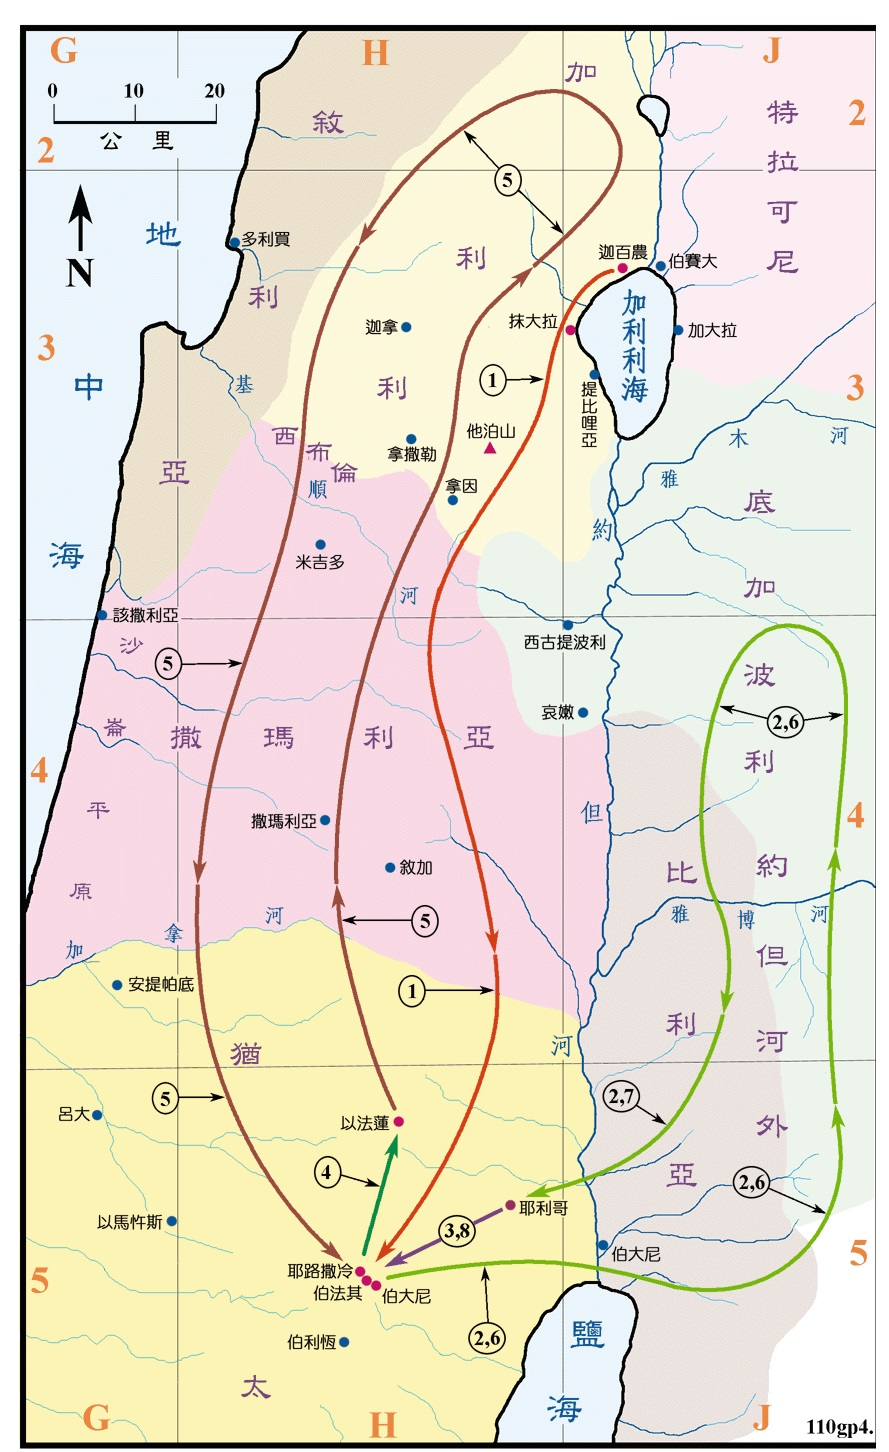
\includegraphics[width=150mm]{ZongJie/SiFuYin/figs/jesustripMinistry2} 
\caption{最后一次去耶路撒冷}
\end{figure}



\begin{table}[H]
  \centering
    \begin{tabular}{p{14em}|p{7.93em}|l|l|l|p{4.855em}}
    \toprule
    \textbf{事 件} & \textbf{地 點} & \multicolumn{1}{p{5.285em}|}{\textbf{馬太福音}} & \multicolumn{1}{p{5.57em}|}{\textbf{馬可福音}} & \multicolumn{1}{p{5.285em}|}{\textbf{路加福音}} & \textbf{約翰福音} \\  \midrule


論進神國要努力進窄門&\textcolor{red}{耶京路過的城鄉}&       &       & \multicolumn{1}{p{5.285em}|}{13:22-30} & \multicolumn{1}{l}{} \\\midrule
對法利賽人論希律殺耶穌之事& 比利亞？   &       &       & \multicolumn{1}{p{5.285em}|}{13:31-33} & \multicolumn{1}{l}{} \\\midrule

論耶路撒冷結局,為其悲哀 & 比利亞？   &       &       & \multicolumn{1}{p{5.285em}|}{13:34-35} & \multicolumn{1}{l}{} \\\midrule


 
耶穌安息日醫治水臌病人 &法利賽首領家&       &       & \multicolumn{1}{p{5.285em}|}{14:1-6} & \multicolumn{1}{l}{} \\ \midrule

警告揀擇首位的客人& 比利亞？   & & & \multicolumn{1}{p{5.285em}|}{14:7-11}& \multicolumn{1}{l}{} \\ \midrule
教訓筵席的主人& 比利亞？   & & & \multicolumn{1}{p{5.285em}|}{14:12-14}& \multicolumn{1}{l}{} \\ \midrule

以大筵席喻猶太人藐視救恩& 比利亞？&&& \multicolumn{1}{p{5.285em}|}{14:15-24} & \multicolumn{1}{l}{} \\ \midrule

從者計算花費,作門徒的代價& 比利亞？   &       &       & \multicolumn{1}{p{5.285em}|}{14:25-35} & \multicolumn{1}{l}{} \\ \midrule


法利賽人文士論主接待稅吏罪人& 比利亞？   & &       & \multicolumn{1}{p{5.285em}|}{15:1-2} & \multicolumn{1}{l}{} \\ \midrule

失羊的比喻 & 比利亞？   &18:12-14       &       & \multicolumn{1}{p{5.285em}|}{15:3-7} & \multicolumn{1}{l}{} \\ \midrule
失錢的比喻 & 比利亞？   & &       & \multicolumn{1}{p{5.285em}|}{15:8-10} & \multicolumn{1}{l}{} \\ \midrule

浪子的比喻 & 比利亞？   &&       & \multicolumn{1}{p{5.285em}|}{15:11-32} & \multicolumn{1}{l}{} \\ \midrule

耶穌設不義聰管家爲喻 & 比利亞？   &       &       & \multicolumn{1}{p{5.285em}|}{16:1-12} & \multicolumn{1}{l}{} \\\midrule
一個僕人不能侍奉兩個主&   &       &       & \multicolumn{1}{p{5.285em}|}{16:13} & \multicolumn{1}{l}{} \\\midrule
责法利賽人自稱為義&   &       &       & \multicolumn{1}{p{5.285em}|}{16:14-17} & \multicolumn{1}{l}{} \\\midrule

%法利賽人試探耶穌休妻条件& 以法蓮？   & \multicolumn{1}{p{5.285em}|}{19:3-6} & \multicolumn{1}{p{5.57em}|}{} &       & \multicolumn{1}{l}{} \\\midrule

%法利賽人惑摩西律法可以休妻& 以法蓮？   & \multicolumn{1}{p{5.285em}|}{19:7-9} & \multicolumn{1}{p{5.57em}|}{10:2-9} &       & \multicolumn{1}{l}{} \\\midrule

%對門徒說休妻另娶的就是犯姦淫& 屋裡 & \multicolumn{1}{p{5.285em}|}{} & \multicolumn{1}{p{5.57em}|}{10:10-12} &       & \multicolumn{1}{l}{} \\\midrule

%主以为天国单身解門徒婚姻之惑& 屋裡  & \multicolumn{1}{p{5.285em}|}{19:10-12} & \multicolumn{1}{p{5.57em}|}{} &       & \multicolumn{1}{l}{} \\\midrule
離開加利利到猶太治病人& \multicolumn{1}{p{7.93em}|}{約旦河外} & \multicolumn{1}{p{5.285em}|}{19:1-2} &10:1 & &\multicolumn{1}{p{4.855em}}{} \\\midrule

法利賽人試探耶穌何故可休妻&猶太境約旦河外 &19:3&10:2& \multicolumn{1}{p{5.285em}|}{} & \multicolumn{1}{l}{} \\\midrule
主答创世记二人成為一體&猶太境約旦河外 &19:4-6&10:6-9& \multicolumn{1}{p{5.285em}|}{} & \multicolumn{1}{l}{} \\\midrule
摩西為何许可給妻子休書&猶太境約旦河外 &19:7-8&10:3-5& \multicolumn{1}{p{5.285em}|}{} & \multicolumn{1}{l}{} \\\midrule

对门徒論休妻另娶的犯姦淫&約旦河外屋裡 & 19:9 &10:10-12& \multicolumn{1}{p{5.285em}|}{16:18} & \multicolumn{1}{l}{} \\\midrule
主以为天国单身解門徒婚姻之惑&約旦河外屋裡  & \multicolumn{1}{p{5.285em}|}{19:10-12} & \multicolumn{1}{p{5.57em}|}{} &       & \multicolumn{1}{l}{} \\\midrule

耶穌論財主與拉撒路 & 比利亞 ？  &       &       & \multicolumn{1}{p{5.285em}|}{16:19-31} & \multicolumn{1}{l}{} \\ \midrule
%使信主小子跌倒的不如去死& \multicolumn{1}{p{7.93em}|}{迦百農} & \multicolumn{1}{p{5.285em}|}{18:6-7} & \multicolumn{1}{p{5.57em}|}{9:42} & &  \\ \midrule
絆倒人有禍不如頸拴石沉海& 迦百農 ？  &  \multicolumn{1}{p{5.285em}|}{18:6-7} & \multicolumn{1}{p{5.57em}|}{9:42}  & \multicolumn{1}{p{5.285em}|}{17:1-2} & \multicolumn{1}{l}{} \\\midrule

一天七次饒恕懊悔的弟兄& 比利亞 ？  &       &       & \multicolumn{1}{p{5.285em}|}{17:3-4} & \multicolumn{1}{l}{} \\\midrule

對使徒論信心與僕人的本分 & 比利亞 ？  &       &       & \multicolumn{1}{p{5.285em}|}{17:5-10} & \multicolumn{1}{l}{} \\\midrule

耶穌使拉撒路由死複生 & 伯大尼   &       &       &       & 11:1-45\\\midrule

祭司長等想要殺死耶穌& 耶路撒冷  &       &       &       & 11:46-57 \\\midrule
耶穌在曠野和那裡門徒同住&以法蓮&       &       &       & 11:54-55\\\midrule
醫十個大痲瘋讚撒瑪利亞人信心&\textcolor{red}{耶京過撒瑪利亞}&       &       & \multicolumn{1}{p{5.285em}|}{17:11-19} & \multicolumn{1}{l}{} \\ \midrule

對法利賽人論神國在人心裡&去耶京的路上&       &       & \multicolumn{1}{p{5.285em}|}{17:20-21} & \multicolumn{1}{l}{} \\ \midrule

對門徒以挪亞羅得論人子再來&去耶京的路上&       &       & \multicolumn{1}{p{5.285em}|}{17:22-32} & \multicolumn{1}{l}{} \\ \midrule

捨生命者得生命&去耶京的路上&       &       & \multicolumn{1}{p{5.285em}|}{17:33-37} & \multicolumn{1}{l}{} \\ \midrule


以切求的寡婦教導禱告要恒切&去耶京的路上&       &       & \multicolumn{1}{p{5.285em}|}{18:1-8} & \multicolumn{1}{l}{} \\ \midrule

法利賽人稅吏禱告,論自義自卑&去耶京的路上&       &       & \multicolumn{1}{p{5.285em}|}{18:9-14} & \multicolumn{1}{l}{} \\\midrule

耶穌惱怒門徒爲孩子祝福 &去耶京的路上？& \multicolumn{1}{p{5.285em}|}{19:13-15} & \multicolumn{1}{p{5.57em}|}{10:13-16} & \multicolumn{1}{p{5.285em}|}{18:15-16} & \multicolumn{1}{l}{} \\\midrule

不回轉成小孩子不得進天國&去耶京的路上？& \multicolumn{1}{p{5.285em}|}{18:3} & \multicolumn{1}{p{5.57em}|}{10:15} & \multicolumn{1}{p{5.285em}|}{18:17} & \multicolumn{1}{l}{} \\\midrule
% \bottomrule
\end{tabular}%
\end{table}%

\begin{table}[H]
  \centering
    \begin{tabular}{p{14em}|p{7.93em}|l|l|l|p{4.855em}}
    \toprule
    \textbf{事 件} & \textbf{地 點} & \multicolumn{1}{p{5.285em}|}{\textbf{馬太福音}} & \multicolumn{1}{p{5.57em}|}{\textbf{馬可福音}} & \multicolumn{1}{p{5.285em}|}{\textbf{路加福音}} & \textbf{約翰福音} \\  \midrule

富足官求永生憂愁而去&出來行路的時候&\multicolumn{1}{p{5.285em}|}{19:16-22}&\multicolumn{1}{p{5.285em}|}{10:17-22}& \multicolumn{1}{p{5.285em}|}{18:18-23} & \multicolumn{1}{l}{} \\\midrule

教導門徒財主靠財難進天國&去耶京的路上& \multicolumn{1}{p{5.285em}|}{19:23-26} & \multicolumn{1}{p{5.57em}|}{10:23-27} & \multicolumn{1}{p{5.285em}|}{18:24-27} & \multicolumn{1}{l}{} \\\midrule

對彼得論門徒從主審判十二支派&去耶京的路上& \multicolumn{1}{p{5.285em}|}{19:27-28} & \multicolumn{1}{p{5.57em}|}{} & \multicolumn{1}{p{5.285em}|}{} & \multicolumn{1}{l}{} \\\midrule

對彼得論今世得百倍來世得永生&去耶京的路上& \multicolumn{1}{p{5.285em}|}{19:29-30} & \multicolumn{1}{p{5.57em}|}{10:28-31} & \multicolumn{1}{p{5.285em}|}{18:28-30} & \multicolumn{1}{l}{} \\\midrule

葡萄園雇工各得一錢銀子之喻 && \multicolumn{1}{p{5.285em}|}{20:1-16} &       &       & \multicolumn{1}{l}{} \\\midrule

耶穌對門徒\textcolor{red}{第四次}提及受害事 &去耶京的路上& \multicolumn{1}{p{5.285em}|}{20:17-19} & \multicolumn{1}{p{5.57em}|}{10:32-34} & \multicolumn{1}{p{5.285em}|}{18:31-34} & \multicolumn{1}{l}{} \\\midrule


雅各约翰母亲为子争左右位&  & \multicolumn{1}{p{5.285em}|}{20:20-23} & \multicolumn{1}{p{5.57em}|}{10:35-40} &       & \multicolumn{1}{l}{} \\\midrule

十個門徒聽見惱怒弟兄二人&   & \multicolumn{1}{p{5.285em}|}{20:24} & \multicolumn{1}{p{5.57em}|}{10:41} &       & \multicolumn{1}{l}{} \\\midrule

對門徒論誰願為首必做僕人&   & \multicolumn{1}{p{5.285em}|}{20:25-28} & \multicolumn{1}{p{5.57em}|}{10:42-45} &       & \multicolumn{1}{l}{} \\\midrule

耶穌醫治兩個瞎子（巴底買） & 耶利哥城外 & \multicolumn{1}{p{5.285em}|}{20:29-34} & \multicolumn{1}{p{5.57em}|}{10:46-52} & \multicolumn{1}{p{5.285em}|}{18:35-43} & \multicolumn{1}{l}{} \\ \midrule

税吏長財主撒該信主  & 耶利哥   &       &       & \multicolumn{1}{p{5.285em}|}{19:1-10} & \multicolumn{1}{l}{} \\  \midrule

對眾人設交銀與十僕喻神國顯现 & 耶利哥   &       &       & \multicolumn{1}{p{5.285em}|}{19:11-27} & \multicolumn{1}{l}{} \\ \midrule

\end{tabular}%
\end{table}%